\chapter{Einführung}
    \section{Properties of Communication} % 1.13
        \begin{itemize}
        	\item Ausbreitungsverzögerung
        	\item Datenrate
        	\item Fehlerrate
        \end{itemize}
    % end

    \section{Simplex}
        In einem Simplex Netz können Daten nur in eine Richtung gesendet werden.
    % end

    \section{Halb-Duplex}
        In einem Halb-Duplex Netz können Daten in beide Richtungen gesendet werden, aber nicht zur gleichen Zeit.
    % end

    \section{Voll-Duplex}
        In einem Voll-Duplex Netz können Daten zur gleichen Zeit in beide Richtungen gesendet werden.
    % end

    \section{Switching}
        \subsection{Verbindungs Switching}
            Es wird eine Verbindung zwischen zwei Endpunkten hergestellt.
        % end

        \subsection{Paket Switching}
            Es werden Pakete versandt und keine Verbindung hergestellt.
        % end
    % end

    \section{Multiplexing}
        Mehrere Sender wollen gleichzeitig Daten über ein Medium senden.

        \subsection{Time Division Multiplexing}
            Die Sender senden nacheinander.
        % end

        \subsection{Frequency Division Multiplexing}
            Die Sender senden zeitgleich auf unterschiedlichen Frequenzen.
        % end

        \subsection{CDM, SDM}
            \begin{description}
            	\item[Code Division Multiplexing] Die Sender senden zeitgleich mit verschiedenen Spreizcodes.
            	\item[Space Division Multiplexing] Die Sender senden zeitgleich über unterschiedliche Medien (räumlich).
            \end{description}
        % end
    % end

    \section{Broadcast Medium}
        Medien, die nur von einem Sender zur gleichen Zeit genutzt werden können (bspw. Kupferleitungen).
    % end

    \section{Netzwerk Typen}
        \subsection{Verbindunsorientiert}
            Die Erste Phase der Kommunikation ist die Herstellung einer Verbindung. Danach sind die Kommunikationspartner verbunden.
        % end

        \subsection{Verbindungslos}
            Es wird keine Verbindung hergestellt und übertragen direkt die Daten.
        % end
    % end
% end

\chapter{OSI Schichtenmodell}
    Das OSI-Schichtenmodell beschreibt ein Standard-Schichtenmodell für Netzwerke und besteht aus 7 Schichten, wobei die oberen drei Schichten nur schwach voneinander abgegrenzt sind und oftmals zusammengefasst werden. Im Internet umgesetzt ist oftmals nur das DoD-Schichtenmodell, welches dem OSI-Schichtenmodell in den unteren vier Schichten gleicht und die oberen drei in einer Schicht zusammenfasst.
    
    Das Schichtenmodell besteht aus den folgenden Schichten, die weiter unten auch noch genauer erläutert werden:
    \begin{figure}[H]
    	\centering
    	\begin{tikzpicture}[layer/.style = { draw, rectangle, minimum width = 4cm, align = center, minimum height = 1.2cm }, transit/.style = { minimum width = 2cm, minimum height = 0.5cm }, virtual/.style = { color = TUDa-0b, text = . }]
        	% Layers Left.
        	\node [layer] (layer1Left) {Physical \\ Layer 1};
        	\node [layer, above = of layer1Left] (layer2Left) {Data Link \\ Layer 2};
        	\node [layer, above = of layer2Left] (layer3Left) {Network \\ Layer 3};
        	\node [layer, above = of layer3Left] (layer4Left) {Transport \\ Layer 4};
        	\node [layer, above = of layer4Left] (layer5Left) {Session \\ Layer 5};
        	\node [layer, above = of layer5Left] (layer6Left) {Presentation \\ Layer 6};
        	\node [layer, above = of layer6Left] (layer7Left) {Application \\ Layer 7};
        	% Transit.
        	\node [layer, transit, right = of layer1Left] (transit1Left) {};
        	\node [layer, transit, right = of layer2Left] (transit2Left) {};
        	\node [layer, transit, right = of layer3Left] (transit3Left) {};
        	\node [layer, transit, right = of transit1Left] (transit1Right) {};
        	% Layers Right.
        	\node [layer, right = of transit1Right] (layer1Right) {Physical \\ Layer 1};
        	\node [layer, above = of layer1Right] (layer2Right) {Data Link \\ Layer 2};
        	\node [layer, above = of layer2Right] (layer3Right) {Network \\ Layer 3};
        	\node [layer, above = of layer3Right] (layer4Right) {Transport \\ Layer 4};
        	\node [layer, above = of layer4Right] (layer5Right) {Session \\ Layer 5};
        	\node [layer, above = of layer5Right] (layer6Right) {Presentation \\ Layer 6};
        	\node [layer, above = of layer6Right] (layer7Right) {Application \\ Layer 7};
        	% Transit continue.
        	\node [layer, transit, left = of layer2Right] (transit2Right) {};
        	\node [layer, transit, left = of layer3Right] (transit3Right) {};
        	
        	% Left.
        	\draw [<->] (layer1Left) -- (layer2Left);
        	\draw [<->] (layer2Left) -- (layer3Left);
        	\draw [<->] (layer3Left) -- (layer4Left);
        	\draw [<->] (layer4Left) -- (layer5Left);
        	\draw [<->] (layer5Left) -- (layer6Left);
        	\draw [<->] (layer6Left) -- (layer7Left);
        	% Right.
        	\draw [<->] (layer1Right) -- (layer2Right);
        	\draw [<->] (layer2Right) -- (layer3Right);
        	\draw [<->] (layer3Right) -- (layer4Right);
        	\draw [<->] (layer4Right) -- (layer5Right);
        	\draw [<->] (layer5Right) -- (layer6Right);
        	\draw [<->] (layer6Right) -- (layer7Right);
        	% Layers <--> Transit.
        	\draw [<->] (layer1Left) -- (transit1Left);
        	\draw [<->, virtual] (layer2Left) -- (transit2Left);
        	\draw [<->, virtual] (layer3Left) -- (transit3Left);
        	\draw [<->] (layer1Right) -- (transit1Right);
        	\draw [<->, virtual] (layer2Right) -- (transit2Right);
        	\draw [<->, virtual] (layer3Right) -- (transit3Right);
        	% Layers Left <--> Layers Right.
        	\draw [<->, virtual] (layer4Left) -- node[above]{Transport Protocol} (layer4Right);
        	\draw [<->, virtual] (layer5Left) -- (layer5Right);
        	\draw [<->, virtual] (layer6Left) -- (layer6Right);
        	\draw [<->, virtual] (layer7Left) -- (layer7Right);
        	% Transit.
        	\draw [<->] (transit1Left) -- (transit2Left);
        	\draw [<->] (transit2Left) -- (transit3Left);
        	\draw [<->] (transit1Right) -- (transit2Right);
        	\draw [<->] (transit2Right) -- (transit3Right);
        	\draw [<->] (transit1Left) -- (transit1Right);
        	\draw [<->, virtual] (transit2Left) -- (transit2Right);
        	\draw [<->, virtual] (transit3Left) -- node[label = {[label distance = 0.2cm]Transit Network}]{} (transit3Right);
    	\end{tikzpicture}
    	\caption{OSI Schichtenmodell}
    	\label{fig:osischichtenmodell}
    \end{figure}
    
    \paragraph{1. Physical Layer}
        \begin{itemize}
        	\item Schicht 1
        	\item Fehleranfälliger (unsicherer) Bit-Strom zwischen physikalisch benachbarten Systemen
        	\item Definitionen von Kabeln, Steckern, \dots
        	\item Protokollbeispiele: RJ-45, RJ-21
        \end{itemize}
    % end
    
    \paragraph{2. Data Link Layer}
        \begin{itemize}
        	\item Schicht 2
        	\item Fehlerbereinigter Strom von Frames zwischen physikalisch benachbarten Systemen
        	\item Pakete sind \enquote{Frames}
        	\item Maximale Framegröße des physikalischen Netzes wird beachtet
        	\item Erkennung (und Bereinigung) von Übertragungsfehlern (Prüfsummen) \\ Nicht alle Systeme bereinigen Fehler, einige Protokolle geben nur weiter, das Fehler passiert sind.
        	\item \textit{Kann} schon Flow Control enthalten (bspw. Sliding Window)
        	\item Protokollbeispiele: Ethernet, WLAN
        \end{itemize}
    % end
    
    \paragraph{3. Network Layer}
        \begin{itemize}
        	\item Schicht 3
        	\item Übertragung von Paketen zwischen entfernten Systemen
        	\item Übernimmt Routing (Wegfindung und Weiterleitung)
        	\item Congestion Control und Flow Control
        	\item Protokollbeispiele: IP, X.25
        \end{itemize}
    % end
    
    \paragraph{4. Transport Layer}
        \begin{itemize}
        	\item Schicht 4
        	\item Logische Verbindung von Prozessen auf entfernten Systemen
        	\item Multiplexing, Paketaufteilung/-zusammenstellung für Schicht 3/5
        	\item Fehlerkorrektur
        	\item Congestion Control und Flow Control
        	\item Abstrahiert Netzwerkdetails und Qualitätsunterschiede im Netzwerk
        	\item Protokollbeispiele: TCP, UDP
        \end{itemize}
    % end
    
    \paragraph{5. Session Layer}
        \begin{itemize}
        	\item Schicht 5
        	\item Logische Verbindung zwischen Prozessen
        	\item Verbindungswiederherstellung nach Fehlern mit sogenannten Checkpoints zur Vermeidung von vollständigen Neuverbindungen
        	\item Protokollbeispiele: X.215, X.225
        \end{itemize}
    % end
    
    \paragraph{6. Presentation Layer}
        \begin{itemize}
        	\item Schicht 6
        	\item Systemunabhängige Darstellung von Daten
        	\item Enthält Datenkompression und Verschlüsselung
        	\item Gewährleistung der syntaktischen Korrektheit bei Sender und Empfänger (Nutzung von ASN.1)
        	\item Protkollbeispiele: X.216, ISO 9576
        \end{itemize}
    % end
    
    \paragraph{7. Application Layer}
        \begin{itemize}
        	\item Schicht 7
        	\item Anwendungen für Endnutzer
        	\item Die Anwendungen gehören selbst nicht zur Schicht, sondern nur die Datenein/-ausgabe
        	\item Anwendungsbeispiele: Browser, E-Mail Programm
        \end{itemize}
    % end
% end

\chapter{Routing}
    Routing beschäftigt sich mit der Pfadfindung von Start zu Ziel und wie Pakete am schnellsten zugestellt werden können.
    \begin{itemize}
    	\item Diese Aufgabe wird auf OSI-Schicht 2 (Network) übernommen, also von IP (o.ä.).
    	\item Zur Pfadfindung werden \textit{Routing Algorithmen} eingesetzt, die den Pfad finden.
    \end{itemize}

    \section{Weiterleitung (Forwarding)}
        Als \textit{Forwarding} wird die Weiterleitung von Paketen bezeichnet, die sich an die von Routing Algorithmen berechnete Route hält. Anders ausgedrückt: Forwarding bezeichnet das simple verschieben eines Paketes von einem Knoten zum nächsten.
        
        Der Routing Algorithmus erstellt dabei eine Routing Tabelle, in der für jeden Knoten (bzw. Netz) steht, an welchen Knoten die Pakete weitergeleitet werden sollen.
        
        \begin{figure}[H]
		    \centering
            \begin{tikzpicture}
	            \ciscoClient{net1}{}{below:Host 1};
	            \ciscoRouter{router1}{right = of net1}{below:Router 1};
	            \ciscoInternet{inet}{right = of router1}{below:Internet};
	            \ciscoRouter{router2}{right = of inet}{below:Router 2};
	            \ciscoClient{net2}{right = of router2}{below:Host 2};
	            
	            \draw (net1) -- (router1);
	            \draw (router1) -- (inet);
	            \draw (inet) -- (router2);
	            \draw (router2) -- (net2);
            \end{tikzpicture}
            \caption{Routing Einleitung}
        \end{figure}
    % end

    \section{Optimierungskriterien}
        \begin{itemize}
        	\item Korrektheit
        	\item Simplizität
        	\item Robustheit
        	\item Fairness
        	\item Optimalität
        \end{itemize}
        
        Diese Ziele konkurrieren oft miteinander und sind nicht alle zur gleichen Zeit umsetzbar.
        
        Zur Bewertung der Algorithmen können folgende Metriken helfen:
        \begin{itemize}
        	\item Durchschnittliche Paketverzögerung
        	\item Gesamte Brandbreite
        	\item Individuelle Verzögerungen
        \end{itemize}
        
        In der Praxis versuchen Routing Algorithmen die Anzahl an Hops pro Paket zu reduzieren. Dies ist nicht immer optimal, aber gut genug.
    % end

    \section{Routing Algorithmen}
        Routing Algorithmen werden klassifiziert in:
        \begin{description}
        	\item[Adaptive Routing Algorithmen] Der Algorithmus passt sich den aktuellen Netzwerkgegebenheiten an (bspw. DVR, LSR, \dots).
        	\item[Nicht-Adaptive Routing Algorithmen] Der Algorithmus passt sich nicht dem Netzwerk an und funktioniert immer gleich (bspw. Flooding).
        \end{description}
        
        \paragraph{Adaptive Routing Algorithmen}
            Adaptive Routing Algorithmen werden in folgende Unterkategorien eingeteilt:
            \begin{description}
            	\item[Zentralisiert] Ein zentraler Knoten steuert das Routing für das gesamte Netzwerk.
	            	\begin{itemize}
	            		\item Die Router teilen regelmäßig ihre Routing Tabellen mit dem zentralen Dienst.
	            		\item Der zentrale Dienst kann die besten Routen berechnen und wieder mit den Routern teilen.
	            		\item Problematiken:
	            		\begin{itemize}
	            			\item Angreifbar: Wenn der zentrale Dienst stirbt, wird das Routing zu einem nicht-adaptivem Routing.
	            			\item Skalierbarkeit: Der Dienst muss sehr viele Informationen bereit halten und viel Traffic behandeln.
	            			\item Flaschenhals: Um das Zentrum herum ist viel Traffic unterwegs.
	            			\item Alterung: Router, die nahe am Zentrum sind bekommen neue Routing Tabellen eher mit als entfernte Router.
	            		\end{itemize}
	            	\end{itemize}
            	\item[Isoliert] Jeder Router entscheidet sich selbst für Wege basierend auf den lokalen Informationen. Es findet kein Nachrichtenaustausch zwischen Routern statt.
            	\item[Verteilt] Die Router kommunizieren regelmäßig miteinander, um die Routing Tabellen zu teilen und zu updaten. \\ Auch diese Art von Routing kann nochmals in unterteilt werden:
	            	\begin{itemize}
	            		\item Dezentrale vs. Globale Informationen
		            		\begin{itemize}
		            			\item Bei dezentraler Informationsverwaltung kennt jeder Knoten nur seine direkten Nachbarn und es werden Informationen mit diesen ausgetauscht. \\ Diese Algorithmen heißen \textit{Distance Vector} Algorithmen.
		            			\item Bei globaler Informationsverwaltung kennt jeder Knoten alle anderen und die Kosten der Kanten, \dots. \\ Diese Algorithmen heißten \textit{Link State} Algorithmen.
		            		\end{itemize}
		            	\item Statische vs. Dynamisch Routen
			            	\begin{itemize}
			            		\item Bei statischen Routen ändern sich diese nur sehr langsam über die Zeit.
			            		\item Bei dynamischen Routen können sich die Routen schnell ändern (bspw. durch periodische Updates oder als Reaktion auf Änderungen im Netzwerk).
			            	\end{itemize}
	            	\end{itemize}
            \end{description}
        % end
        
        \subsection{Flooding [Nicht Adaptiv]}
	        \begin{itemize}
	        	\item Standard-Algorithmus für nicht-adaptive Algorithmen.
	        	\item Die Pakete werden nicht geroutet sondern einfach über das gesamte Netzwerk versendet (es wird geflutet).
	        	\item \textbf{Problematik:} Es werden sehr viel mehr Pakete versendet als nötig.
	        	\item Strategien zur Verringerung der duplizierten Pakete:
	        	\begin{enumerate}
	        		\item Einen Time-To-Life Wert im Header mitführen, der bei jedem Schritt um 1 reduziert wird. Ist der Wert Null, so wird das Paket verworfen.
	        		\item Router behalten die Sequenznummer der bereits weitergeleiteten Pakete und leiten keine Pakete weiter, die bereits weitergeleitet wurden.
	        	\end{enumerate}
	        	\item Flooding ergibt Sinn, wenn:
	        	\begin{itemize}
	        		\item das Netzwerk sich schnell ändert und adaptives Routing zu langsam wäre oder
	        		\item viele oder alle Pakete Multicast Pakete sind und die Pakete somit ohnehin dupliziert werden.
	        	\end{itemize}
	        \end{itemize}
        % end
        
        \subsection{Hot Potato [Nicht Adaptiv]}
	        \begin{itemize}
	        	\item Eingehende Pakete werden so schnell wie möglich weiter gesendet.
	        	\item \textbf{Problematik:} Manche Pakete kommen erst sehr spät oder nie an.
	        	\item Allerdings wird Hot Potato Routing dennoch oft eingesetzt (bspw. um Mitglieder im Netzwerk zu erkennen).
	        \end{itemize}
        % end
        
        \subsection{Statisches Routing [Nicht Adaptiv]}
	        \begin{itemize}
	        	\item Alle Router werden \enquote{von Hand} vorkonfiguriert mit allen möglichen Zielen.
	        	\item Dies funktioniert sehr gut in statischen Umgebungen.
	        	\item \textbf{Problematik:} Im allgemeinen ändern sich Netzwerke regelmäßig, statisches Routing kann hiermit nicht arbeiten.
	        	\item \textbf{Problematik:} Wenn der Traffic sehr stark schwankt, kann mit nicht-adaptivem Routing keine bessere Route gefunden werden, da sich der Algorithmus nicht anpasst.
	        \end{itemize}
        % end
        
        \subsection{Backward Learning Routing [Adaptiv, Isoliert]}
            \begin{itemize}
            	\item Grundidee
	            	\begin{itemize}
	            		\item Die Quelladresse und ein Hop Counter befinden sich im Header.
	            		\item Anhand dieser Daten lernt der Algorithmus Dinge über das Netzwerk, indem Pakete verarbeitet werden.
	            	\end{itemize}
	            \item Algorithmus
		            \begin{enumerate}
		            	\item Initialisiere alle Router mit einer leeren Routing Tabelle.
		            	\item Starte mit zufälligem Routing (Hot Potato oder Flooding).
		            	\item Für jedes Paket tue:
			            	\begin{enumerate}
			            		\item Wenn Hop Count = 1
				            	   \\ \(\rightarrow\) Das Paket kommt direkt von einem Nachbarn.
				            	   \\ \(\rightarrow\) Nachbarn werden über ihre Verbindung identifiziert.
				            	\item Wenn Hop Count > 1
				            	   \\ \(\rightarrow\) Die Quelle ist \(n\) Hops entfernt.
			            	\end{enumerate}
			            \item Wird ein Paket gefunden, dessen Hop Count in Kombination mit der Quelle kleiner ist als alle vorherigen, wurde eine bessere Route gefunden
			               \\ \(\rightarrow\) Passe die Routing Tabelle entsprechend an.
		            \end{enumerate}
            \end{itemize}
            \begin{figure}[H]
            	\centering
            	\begin{lstlisting}
Initialize all Routers with empty Routing Table;
Start with Random Routing (Hot Potato or Flooding);
            	\end{lstlisting}
            	\caption{Backward Learning Routing}
            \end{figure}
        % end

        \subsection{Distance Vector Routing [Adaptiv, Verteilt, Dezentrale Info]}
            \begin{itemize}
            	\item Es werden Nachrichten mit den Nachbarn ausgetauscht und die Informationen aggregiert.
            	\item Iterativ: Das Verfahren läuft so lange, bis keine Verbesserungen mehr auftreten. Dann stoppen die Knoten die Kommunikation (Selbstterminierend).
            	\item Verteilt: Jeder Knoten kommuniziert nur mit seinen direkten Nachbarn und kennt nur deren Zustand.
            \end{itemize}
            
            \paragraph{Struktur der Distanztabelle}
                \begin{itemize}
                	\item Jeder Knoten hat eine Zeile für jedes mögliche Ziel.
                	\item Jeder Knoten hat eine Spalte für jeden Nachbarn.
                	\item Distanz (in Knoten X, mit Ziel Y über Nachbar Z): \( D ^ X (Y, Z) = c(X, Z) + \min _ w { D ^ Z (Y, w) } \)
                	\item Anschließend kann die Routing Tabelle einfach abgelesen werden, indem in jeder Zeile die Spalte mit dem geringsten Wert gewählt wird.
                \end{itemize}
            % end
            
            \paragraph{Algorithmus}
                \begin{itemize}
                	\item Jede \textit{lokale Iteration} wird verursacht durch:
	                	\begin{itemize}
	                		\item Eine Änderung der Kosten oder
	                		\item Einer Nachricht von einem Nachbarn.
	                	\end{itemize}
	                \item Jeder Knoten benachrichtigt seine Nachbarn, wenn sich mindestens ein Pfad geändert hat. \\ Die Nachbarknoten wiederum benachrichtigen ihre Nachbarknoten nur, wenn sich ihre Tabelle geändert hat.
	                \item \textbf{Problematik:} Schlechte Nachrichten wandern langsam durch das Netz und können zum \enquote{Count-to-Infinity}-Problem führen (eine Verbindung zählt \enquote{bis} unendlich).
                \end{itemize}
                
                \textbf{Initialisierung Knoten X:}
                \begin{figure}[H]
                	\centering
                	\begin{lstlisting}
for all neighbours v:
	*@\(D^X\)@*(*, v) = *@\(\infty\)@*
	*@\(D^X\)@*(*, v) = c(X, v)
rof

for all destinations y:
	send min*@\(_w D^X\)@*(y, w) to each neighbour
rof
                	\end{lstlisting}
                	\caption{DVR: Initialisierung Knoten X}
                \end{figure}
                
                \textbf{Schleife Knoten X:}
                \begin{figure}[H]
                	\centering
                	\begin{lstlisting}
forever:
	wait (link cost change to neighbour V or update from neighbour V)

	if (c(X, V) changed by d):
		for all destinations y:
			*@\(D^X\)@*(y, V) = *@\(D^X\)@*(y, V) + d
	else if (update received from V with destination Y):
		let newval = min*@\(_w D^V\)@*(Y, w) received from update
		*@\(D^X\)@*(Y, V) = c(X, V) + newval
	fi

	if (new min*@\(_w D^X\)@*(Y, w) for any destination Y):
		send min*@\(_w D^X\)@*(Y, w) to each neighbour
	fi
reverof
                	\end{lstlisting}
                	\caption{DVR: Schleife Knoten X}
                \end{figure}
            % end

            \subsubsection{Poisened Reverse}
                \begin{itemize}
                	\item Posened Reverse ist eine Lösung des Count-to-Infinity Problems in kleinen Netzen.
                	\item In großen Netzen kann das Problem dennoch auftreten.
                	\item \textbf{Funktionsweise:} Erhöhen sich die Link-Kosten, so benachrichtigt ein Knoten die Nachbarn und tut dabei so, als sei er gestoben. Das heißt, er teilt den Nachbarknoten mit, eine Verbindung dauere unendlich lange.
                	\item Da gute Nachrichten sich schnell durch das Netzwerk verbreiten, wird die Unerreichbarkeit sobald wie möglich aufgehoben.
                \end{itemize}
                
                \textit{Kommentar: Bei diesem Abschnitt bin ich mir unsicher, ob die Informationen so korrekt sind.} \todo{Understand}
            % end

            \subsubsection{Split Horizon}
                \begin{itemize}
                	\item Split Horizon ist ähnlich zu Poisened Reverse und versucht, das gleiche Problem zu lösen.
                	\item \textbf{Idee:} Geänderte Routen nicht an Nachbarn weitergeben, der das Update ausgelöst hat.
                	\item Hierdurch wird das Count-to-Infinity Problem effektiv behoben.
                \end{itemize}
            % end
        % end

        \subsection{Link-State Routing [Adaptiv, Verteilt, Globale Info]}
			\begin{itemize}
				\item Die Routen werden effizient mittels Dijkstra gefunden.
				\item Jeder Knoten und jede Kante sind jedem Knoten bekannt.
				\item Diese Informationen werden mittels Broadcasts im Netzwerk bekannt gegeben.
				\item Dabei sendet jeder Router die Kosten zu seinen Nachbarn an seine Nachbarn (Flooding). \\ Bereits bekannte Pakete oder abgelaufene werden verworfen, die anderen Pakete werden weitergeleitet.
				\item Sobald alle Pakete bekannt sind, wird die Topologie konstruiert und Dijkstra ausgeführt.
			\end{itemize}
        % end

        \subsection{Vergleich DVR \(\leftrightarrow\) LSR}
            \begin{itemize}
            	\item Nachrichtenkomplexität
	            	\begin{description}
	            		\item[DVR] Austausch nur zwischen den Nachbarn
	            		\item[LSR] Mit \(n\) Knoten und \(E\) Kanten: \(\mathcal{O}(m \cdot E)\) Nachrichten pro Runde.
	            	\end{description}
            	\item Konvergenzgeschwindigkeit
	            	\begin{description}
	            		\item[DVR] Kann Schleifen enthalten, Count-to-Infinity Problem
	            		\item[LSR] \(\mathcal{O}(n^2)\) Algorithmus benötigt \(\mathcal{O}(n \cdot E)\) Nachrichten, kann Schwingungen enthalten
	            	\end{description}
            	\item Robustheit (Was passiert, wenn ein Router nicht funktioniert?)
	            	\begin{description}
	            		\item[DVR] Knoten können inkorrekte Pfad-Kosten verteilen, jede Tabelle wird von jedem anderen Knoten verwendet \(\implies\) Der Fehler wird durch das gesamte Netz propagiert.
	            		\item[LSR] Knoten können inkorrekte Link-Kosten verteilen, jeder Knoten hat eine eigene Tabelle \(\implies\) Der Fehler wird nicht propagiert.
	            	\end{description}
            \end{itemize}
        % end

        \subsection{Hierarchisches Routing}
            \begin{itemize}
            	\item Bisher wird von flachem Routing ausgegangen.
            	\item In großen Netzwerken skaliert dies allerdings nicht, weshalb hierarchisches Routing eingesetzt werden sollte.
                	\begin{itemize}
                		\item Aufgrund der schieren Anzahl an Knoten ist eine Routing Tabelle der Größe nicht möglich, sie würde die Router abschießen.
                	\end{itemize}
                \item Administrativ gesehen ist das Internet ein Netzwerk von Netzwerken.
                \item Jeder Administrator möchte das Routing in seinem Netz selbst kontrollieren können.
            \end{itemize}

            \subsubsection{Autonome Systemen (AS)}
                \begin{itemize}
                	\item Das globale Internet besteht aus vielen \textit{Autonomen Systemen} (AS), welche untereinander Verbunden sind.
                    	\begin{description}
                    		\item[Stub AS] Kleine Organisationen, nur ein Link ins Internet
                    		\item[Multihomed AS] Große Organisationen, mehrere Links ins Internet
                    		\item[Transit AS]: Provider
                    	\end{description}
                    \item Jedes AS hat eine eindeutige ID.
                    \item Jedes AS muss eine Route in jedes andere AS kennen.
                    \item Autonome Systeme aggregieren Router in Regionen.
                    \item Router in einem AS laufen mit dem selben Routing Protokoll. In unterschiedliche AS können unterschiedliche Routing Protokolle verwendet werden.
                    \item \textit{Gateway Router} sind spezielle Router in einem AS, die das Routing zwischen den AS steuern.
                \end{itemize}
            % end

            \subsubsection{Intra-AS/Inter-AS}
                \begin{itemize}
                	\item Intra-AS: Routing innerhalb eines AS und Routing von Paket nach außen (zum Inter-AS)
                    	\begin{itemize}
                    		\item Routing Information Protocol (RIP): Distance Vector
                    		\item Open Shortes Path First (OSPF): Link State
                    		\item Interior Gateway Routing Protocol (IGRP): Distance Vector (Cisco-Proprietär)
                    	\end{itemize}
                	\item Inter-AS: Routing zwischen verschiedenen AS und Routing von Paketen nach innen (zu Intra-ASs)
                    	\begin{itemize}
                    		\item Border Gateway Protocol (BGP): Path Vector \\ Ähnlich wie Distance Vector, nur mit Schleifenvermeidung etc.
                    	\end{itemize}
                \end{itemize}
            % end
        % end

        \subsection{Border Gateway Protocol (BGP)}
            \begin{itemize}
            	\item Der Standard beim Inter-AS Routing
            	\item Erhält die Information, wie welche Subnetze innerhalb eines AS erreicht werden können.
            	\item Propagiert diese an andere AS weiter.
            	\item Baut \enquote{gute} Routen zu Subnetzen basierend auf den vorherigen Informationen.
            	\item Erlaubt Subnetzen, sich anzukündigen (\enquote{Halle, ich bin hier!}).
            \end{itemize}
            
            \paragraph{Grundlagen}
                \begin{itemize}
                	\item BGP Peers tauschen Routing Informationen aus über TCP Verbindungen (BGP Sessions).
                	\item Prefixes können bei einer Bekanntmachung zusammengeführt werden.
                	\item Die Prefixe werden den Gateway Routern registriert, welche diese dann im Inter-AS propagieren.
                \end{itemize}
            % end
            
            \paragraph{Attribute und Routen}
                \begin{itemize}
                	\item Wenn ein Prefix propagiert wird, so enthält die Nachricht den Prefix selbst und Attribute, was zusammen eine Route ergibt.
                	\item Die zwei wichtigsten Attribute sind:
	                	\begin{description}
	                		\item[AS-PATH] Enthält das AS, durch welches die Nachricht gelaufen ist.
	                		\item[NEXT-HOP] Enthält den nächsten Intra-AS Router, um zum nächsten AS zu kommen (dies können mehrere Links sein).
	                	\end{description}
	                \item Ein Gateway nutzt \textit{Import Policies}, um zu entscheiden, ob eine Route angenommen oder verworfen wird.
                \end{itemize}
            % end

            \subsubsection{Skalierung}
                \begin{itemize}
                	\item Die steigende Anzahl an AS ist ein Problem.
                	\item Die Anzahl klein zu halten und dafür die Größe der AS zu erhöhen ist aber auch keine Lösung.
                	\item Dies würde zu hohen Routing Zeiten innerhalb von ASen führen.
                	\item Auf großer Sich beeinflusst das Verhalten eines Routers alle anderen.
                	\item Dies kann zu folgenden Problemen führen:
                    	\begin{itemize}
                    		\item Suboptimales Routing
                    		\item Instabilität der Routen
                    		\item Schwingungen innerhalb einer Route
                    	\end{itemize}
                \end{itemize}
            % end

            \subsubsection{Security} % 2.75, 2.81, 2.82, 2.83, 2.84, 2.85
                \begin{description}
                	\item[Quellen] Untergrabene Router oder Links.
                	\item[Konsequenzen]
                    	\begin{itemize}
                    		\item Falsche Routing Informationen
                    		\item Täuschung von normalen Routern
                    		\item Störung der normalen Routerfunktionen
                    		\item Kompromittierung von Routern (bspw. um Traffic mitzulesen)
                    	\end{itemize}
                    \item[Konsequenzbereiche] Einzelne Knoten bis zum gesamten Internet
                    \item[Konsequenzdauer] Nur während der Attacke bis zu sehr langen Zeitperioden
                \end{description}
                
                \textit{Hier fehlen einige Inhalte der Vorlesung, siehe Kapitel 2: Routing, Folie 81 bis 85.}
            % end
        % end
    % end
    
    \section{Mobile Routing}
        Siehe \ref{c:mobilenetworks}.
    % end
    
    \section{Overlay Routing}
        \begin{itemize}
        	\item Overlay Netzwerke sind sehr populär geworden.
	        	\begin{itemize}
	        		\item Alle P2P-Netzwerke nutzen Overlay Netzwerke.
	        		\item Die meisten Cloud-Speicher nutzen Overlay Netzwerke.
	        	\end{itemize}
	        \item Ein \textit{Overlay Netzwerk} ist eine virtuelle Netzwerktopologie, die das darunterliegende Netzwerk versteckt (abstrahiert).
	        \item Nachbarn in einem Overlay Netzwerk sind nicht unbedingt Nachbarn im darunterliegenden Netz.
	        \item Im Prinzip funktioniert Routing in einem Overlay Netzwerk nicht anders als in einem normalen IP Netzwerk.
	        \item Doch es müssen einige Metriken beachtet werden, ob das Overlay Netzwerk noch effizient ist:
		        \begin{itemize}
		        	\item Die Hops im Overlay Netzwerk.
		        	\item Die Hops im Underlay Netzwerk.
		        	\item Der sogenannte \textit{Stretchfaktor}: (\( \frac{\text{Hops im Underlay Netzwerk}}{Hops im Overlay Netzwerk} \))
		        \end{itemize}
        \end{itemize}
    % end
% end
            
\chapter{Mobile Netzwerke}
    \label{c:mobilenetworks}

    In mobilen Netzen ist oftmals keine Infrastruktur vorhanden, sodass das Routing ein großes Problem wird (es kann nicht einfach alles über einen Knoten geleitet werden, also muss jeder Knoten Pakete weiterleiten können). In diesem Kontext geht es um Ad-Hoc Netzwerke, also nicht um UMTS oder ähnliches, wo eine zentrale Infrastruktur verfügbar ist. Außerdem ändert sich mobile Infrastruktur kontinuierlich, somit somit müssen sich die Routing-Algorithmen schnell an neue Netzwerke anpassen können. Außerdem ändert sich, bedingt durch das Übertragungsmedium der Radiowelle, andauernd die Verbindungsqualität zwischen den Knoten.
    
    \begin{description}
    	\item[Proaktive Verfahren] Die Route wird festgestellt, bevor ein Paket versendet wird.
    	\item[Reaktive Verfahren] Die Route wird während der Zustellung des Paketes festgestellt.
    \end{description}
    
    \section{Routing}
	    Traditionelle Algorithmen wie DVR oder LSR funktionieren nicht sehr gut in mobilen Netzwerken, da sie folgende Eigenschaften eines mobilen Netzes nicht gut behandeln:
	    \begin{itemize}
         	\item Mobile Netze sind sehr \textit{dynamisch},
         	\item durch andauernde Routing-Nachrichten nimmt der \textit{Stromverbrauch} zu,
         	\item die \textit{Bandbreite} zwischen den Knoten ist stark begrenzt,
         	\item durch sehr unterschiedliche Knoten ist die Bandbreite \textit{asymmetrisch} ($ A \rightarrow B $ kann schneller sein als $ A \leftarrow B $),
         	\item die Verbindung kann durch andere Knoten \textit{gestört} werden und
         	\item mobile Netze haben meist eine hohe \textit{Redundanz}, da ein Knoten mit vielen anderen Verbunden sein kann.
	    \end{itemize}
	    
	    Im folgenden werden folgende mobile Routing-Algorithmen behandelt:
	    \begin{itemize}
         	\item Destination Sequenced Distance Vector (DSDV), ein proaktiver Algorithmus und
         	\item Dynamic Source Routing (DSR), ein reaktiver Algorithmus.
	    \end{itemize}
	    
	    \subsection{Destination Sequenced Distance Vector}
		    DSDV ist eine Erweiterung des DVR-Algorithmus um mit mobilen Netzen zu arbeiten (annahmen über die Vermeidung des Count-to-Infinity-Problems funktionieren nicht in mobilen Netzen!).
		    
		    Folgende Erweiterungen sind möglich, damit DVR in mobilen Netzen funktioniert:
		    \begin{enumerate}
		    	\item Sequenznummern für alle Routing Updates
			    	\begin{itemize}
			    		\item Diese sichern eine geordnete Abarbeitung der Updates
			    		\item Vermeidet Schleifen und Inkonsistenzen
			    	\end{itemize}
		    	\item Geringere Update-Frequenz
			    	\begin{itemize}
			    		\item Speicherung der Zeit zwischen \textit{erster} und \textit{bester} Bekanntmachung eines Pfades
			    		\item Sperrung von Updates wenn die gespeicherten Zeiten unsicher wirken
			    	\end{itemize}
		    \end{enumerate}
		    
		    Ist DSDV noch immer proaktiv und leider auch keine wirkliche Verbesserung im Vergleich zu DVR in mobilen Netzen.
	    % end
	    
	    \subsection{Dynamic Source Routing}
		    DSR ist nach folgenden Grundsätzen designt worden:
		    \begin{itemize}
		    	\item Spaltung von Routing in Pfadfindung und Pfadverwaltung
		    	\item Vermeidung von periodischen Updates
		    	\item Unterstützung von statischen und dynamischen Netzwerken mit ca. 200 Knoten (skalierbar)
		    	\item Der Sender findet den Weg eines Paketes
		    \end{itemize}
		    
		    \paragraph{Pfadfindung}
			    \begin{itemize}
			    	\item Die Pfadfindung wird nur ausgeführt, wenn es wirklich benötigt wird und noch keine Route bekannt ist.
			    	\item Nutzung von Flooding und Broadcasts mit \textit{Zieladresse} und \textit{ID}.
				    	\begin{itemize}
				    		\item Flooding ist im allgemeinen sehr Aufwändig, wird allerdings auch nur selten ausgeführt (bei dem ersten Verbindungsaufbau).
				    	\end{itemize}
			    	\item Wenn ein Knoten ein solches Broadcast-Paket erhält, dann:
				    	\begin{enumerate}
				    		\item Wurde bereits ein Paket mit der gleichen ID empfangen? \\ \( \implies \) Paket verwerfen.
				    		\item Ist die eigene Adresse gleich der Zieladresse? \\ \( \implies \) Paket zum Sender zurück senden (der Pfad wird im Paket gehalten).
				    		\item Ansonsten \\ \( \implies \) Eigene Adresse an das Paket anhängen und Broadcasten.
				    	\end{enumerate}
				    \item Am Ende erhält der Sender ein Paket, welches den Pfad zum Ziel enthält.
				    \item Sind bidirektionale Verbindungen nicht garantiert, so muss das Paket mit Flooding zurück geschickt werden.
				    \item \textbf{Optimierungen}
					    \begin{enumerate}
					    	\item Statt nur einer ID zusätzlich einen Counter mitsenden, der in jedem Schritt erhöht wird.
						    	\begin{itemize}
						    		\item Ist der maximale Durchschnitt des Netzwerkes bekannt, kann ein Paket verworfen werden, wenn der Counter größer als der maximale Durchschnitt ist.
						    	\end{itemize}
						    \item Cachen der Pfade von vorbeikommenden Paketen.
							    \begin{itemize}
							    	\item Im Normalfall würden Knoten nur Pfade lernen, wenn sie Pakete senden.
							    	\item Während dem Weiterleiten anderer Pakete können diese gecachet werden.
							    \end{itemize}
					    \end{enumerate}
			    \end{itemize}
		    % end
		    
		    \paragraph{Pfadverwaltung}
			    \begin{itemize}
			    	\item Die Pfadverwaltung wird nur ausgeführt, wenn ein bestehender Pfad genutzt werden soll.
			    	\item Ungenutzte Pfade werden aus der Routing-Tabelle entfernt
			    	\item Nach Absenden eines Paketes führt ein Knoten einen der folgenden Schritte zur Instandhaltung aus:
				    	\begin{enumerate}
				    		\item Warten auf 2 ACKs (wenn möglich, beispielsweise im normalen WLAN).
				    		\item Carrier-Sense: Abwarten, ob andere Knoten das Paket weiterleiten (nicht möglich bei bspw. Richtfunk)
				    		\item Explizites Anfragen eines ACKs
				    	\end{enumerate}
			    	\item Wenn ein Problem aufgetreten ist, wird entweder der Sender darüber informiert oder ein neuer Weg gesucht (Pfadfindung).
			    \end{itemize}
		    % end
		% end
    % end
    
    \section{Clustering}
	    \begin{itemize}
	    	\item Auch in mobilen Netzen kann hierarchisches Routing sinnvoll sein.
	    	\item Hierbei werden benachbarte Knoten in einen Cluster zusammengefasst.
	    	\item Die Grundidee ist, in einem \enquote{intra}-Cluster proaktives Routing zu verwenden und in einem \enquote{inter}-Cluster reaktives Routing zu verwenden.
	    	\item Dies hat folgende Vorteile:
		    	\begin{itemize}
		    		\item In einem kleinen Knoten ist es möglich, alle Knoten zu kennen $ \implies $ Proaktives Routing ist möglich.
		    		\item Bei vielen Clustern gibt es unter diesen Clustern gibt es quasi keine Kommunikation $ \implies $ Reaktives Routing funktioniert besser.
		    	\end{itemize}
	    \end{itemize}
	    
	    \warning{Clustering in dieser Form funktioniert nur, wenn die Knoten innerhalb der einzelnen Cluster die Cluster nicht andauernd wechseln.}
    % end
% end

\chapter{Inter-Networking}
	Das \textit{Internet Protocol} (IP) befindet sich auf OSI-Schicht 3 (Network) und stellt ein Verbindungsloses Protokoll dar, auf welchem höhere Protokolle wir TCP und UDP aufsetzen. Es beschäftigt sich mit dem Routing der Pakete, Subnetting, NATing und vielem mehr.

    \section{Datagramme}
        Bei IP wird von sogenannten \textit{Datagrammen} gesprochen, welche die einzelnen Übertragungseinheiten darstellen (dies ist auf Ethernet-Ebene ein \enquote{Frame} und auf TCP-Ebene in \enquote{Paket}). Allerdings wird, trotz der klaren Namensgebung, häufig von IP-Paketen geredet, weshalb in diesem Kontext \enquote{Datagramm} und \enquote{Paket} synonym aufgefasst wird.
    % end

    \section{IPv4 Paketformat}
        \begin{figure}[H]
        	\centering
            \begin{bytefield}[bitwidth = 1.2em]{32}
	            \bitheader{0-31} \\
	            \begin{rightwordgroup}{Header}
		            \bitbox{4}{Version} & \bitbox{4}{IHL} & \bitbox{8}{ToS} & \bitbox{16}{Total Length} \\
		            \bitbox{16}{Identification} & \bitbox{3}{Flags} & \bitbox{13}{Fragment Offset} \\
		            \bitbox{8}{TTL} & \bitbox{8}{Protocol} & \bitbox{16}{Header Checksum} \\
		            \bitbox{32}{Source Address} \\
		            \bitbox{32}{Destination Address} \\
		            \bitbox{26}{Options \textit{(optional)}} & \bitbox{6}{Padding}
		        \end{rightwordgroup} \\
		        \begin{rightwordgroup}{Body}
		            \bitbox[trl]{32}{} \\
		            \bitbox[rl]{32}{Data} \\
		            \bitbox[rbl]{32}{}
		        \end{rightwordgroup}
            \end{bytefield}
            \caption{IPv4 Paketformat}
            \label{fig:ipv4packet}
        \end{figure}
        
        \begin{description}
        	\item[Version] 4 Bit breit. Die IP-Version. Kann 4 oder 6 sein (IPv4 bzw. IPv6).
        	\item[IHL (Internet Header Length)] 4 Bit breit. Die Gesamtlänge der Kopfdaten in 32 Bit Worten. Somit kann der Header maximal $ (2 ^ 4 - 1) = 15\text{ Worte} $ lang sein.
        	\item[ToS (Type of Service)] 8 Bit breit. Gibt die Priorisierung des Pakets an, wobei RFC 791, RFC 2474 und RFC 3168 zu teilen widersprüchlich sind und nur beide erfüllt sind, wenn die ersten 6 Bit 0 sind.
        	\item[Total Length] 16 Bit breit. Die Gesamtlänge des Paket (inklusive Kopfdaten) in Byte. Somit kann das Paket maximal $ 2 ^ 16 - 1 = 65535\text{ Byte} \approx 64\text{KiB} $ lang sein.
        	\item[Identification] 16 Bit breit. Eindeutige Identifikationsnummer, welche zur Zusammensetzung von zusammengehörigen Paket dient (in Verbindung mit den Feldern \textit{Flags} und \textit{Fragment Offset}).
        	\item[Flags] 3 Bit breit. Mit DF (Don't Fragment) und MF (More Fragments) wird angezeigt, ob ein Paket fragmentiert ist und weitere Fragmente folgen (MF) oder es nicht fragmentiert werden darf (DF).
        	\item[Fragment Offset] 13 Bit breit. Gibt (unabhängig von der Fragmentierung) an, welche Position innerhalb des fragmentierten Paketes durch das erste Byte in dem Datagramm dargestellt wird. Die Angabe erfolgt in 64 Bit Worten und ist unabhängig von der Fragmentierung, wodurch das Paket mehrmals hintereinander fragmentiert werden kann. Ist das Paket nicht fragmentiert, ist das Feld 0.
        	\item[TTL (Time to Life)] 8 Bit breit. Gibt die Lebensdauer des Paketes an, bevor es verworfen wird (sobald TTL = 0). Der Wert des Feldes wird bei jedem Hop um eins verringert.
        	\item[Protocol] 8 Bit breit. Gibt das darunterliegende Protokoll (bspw. TCP) an.
        	\item[Header Checksum] 16 Bit breit. Die Prüfsumme über die Kopfdaten. Zur Berechnung wird das Feld auf 0 gesetzt und der Header in 16 Bit Worte unterteilt. Für die weitere Berechnung siehe \ref{sec:checksumonescomplement}.
        	\item[Source Address] 32 Bit breit. Die Quelladresse.
        	\item[Destination Address] 32 Bit breit. Die Zieladresse.
        	\item[Options and Padding \textit{(optional)}] 0 bis 40 Byte breit. Bis zu 40 Byte an Optionen, wobei verbleibende Bytes bis zum nächsten 32 Bit Wort mit Nullen aufgefüllt werden (Padding).
        	\item[Data] Die Nutzdaten des Paketes.
        \end{description}
    % end

    \section{Adressierung}
        Da flaches Adressieren mittels MAC-Adressen nicht auf große Netzwerke skaliert (es gibt zu viele Geräte und es müsste für jedes Gerät eine Routing-Tabelle vorgehalten werden), hat IP eigene Adressen, welche hierarchisch (bzw. topologisch) strukturiert sind (in sogenannte Netze).
        
        Eine IP Adresse ist eine Folge von 32 Bits, wobei jedes \textit{Interface} eine solche zugewiesen bekommt. Ein Interface ist eine Netzwerkschnittstelle und ein Knoten kann mehrere Interfaces haben (folglich mehrere IP-Adressen), dies ist zum Beispiel bei Routern üblich, welche die Interfaces dann verbinden und die Pakete zwischen diesen weiterleiten.
        
        Da es sehr anstrengend wäre, IP Adressen immer in binär (oder dezimal) anzugeben, werden sie in vier 8 Bit Blöcke unterteilt, welche mit einem Punkt getrennt Dezimal aufgeschrieben werden:
        \begin{align*}
        	                 & \quad\texttt{10101010101000001001011010001100}    \\
        	\rightsquigarrow & \quad\texttt{10101010.10100000.10010110.10001100} \\
        	\rightsquigarrow & \quad\textbf{\texttt{170.160.150.140}}
        \end{align*}
        
        \subsection{Netzmaske}
            Eine IP Adresse enthält immer einen \textit{Netzanteil} und einen \textit{Hostanteil} und die Größe des Netzanteils wird mittels einer \textit{Netzmaske} angegeben. Dabei ist der Netzanteil vorne in der IP Adresse und \( n \) Bits lang, wobei \( n \) durch die Netzmaske festgelegt wird. Die restlichen \( 32 - n \) Bits stellen dann den Hostanteil dar. Für die Netzmaske kann entweder das \( n \) angegeben werden (Kurzschreibweise) oder eine \enquote{IP Adresse}, welche nur vorne 1en hat. Die Anzahl der 1en ist das gleich dem \( n \).
            \begin{table}[H]
            	\centering
            	\begin{tabular}{c | c | c | c | c | c}
            		\# & IP Adresse & Netzmaske & Netzmaske (kurz) & Netzanteil & Hostanteil \\
            		\hline
            		1 & \texttt{192.168.178.2} & \texttt{255.255.255.0} & \texttt{24} & \texttt{192.168.178.0} & \texttt{0.0.0.2} \\
            		2 & \texttt{130.83.40.233} & \texttt{255.255.255.0} & \texttt{24} & \texttt{130.83.40.0} & \texttt{0.0.0.233}
            	\end{tabular}
            	\caption{IP Adressen, Netzanteil, Hostanteil und Netzmaske}
            \end{table}
            Um gleichermaßen eine vollständige IP Adresse als auch die Netzmaske anzugeben, wir diese mit einem Slash getrennt hinter die IP Adresse geschrieben: \texttt{192.168.178.2/24}.
        % end
        
        \subsection{Klassen}
            Um weltweit IP Adressen an Firmen oder kleinere Unternehmen zu vergeben, wurden die IP Adressen in die folgenden Klassen aufgeteilt:
            \begin{description}
            	\item[Class A] Für sehr große Organisationen, nur 255 Netze und 16.000.000 Hosts pro Netz.
            	\item[Class B] Für große Organisationen, 65.000 Netze und 65.000 Hosts pro Netz.
            	\item[Class C] Für kleine Organisationen, 16.000.000 Netze und 255 Hosts pro Netz.
            	\item[Class D] Multicastadressen, keine Netz/Host Hierarchie.
            	\item[Class E] Reserviert.
            \end{description}
            Ferner wurden für die Netze folgende Eigenschaften festgelegt, damit die Netze von Routern und Menschen voneinander unterschieden werden können:
            \begin{description}
            	\item[Class A] { \begin{bytefield}{32} \bitbox{1}{\texttt{0}} & \bitbox{7}{Net} & \bitbox{24}{Host} \end{bytefield} }
            	\item[Class B] { \begin{bytefield}{32} \bitbox{2}{\texttt{10}} & \bitbox{14}{Net} & \bitbox{16}{Host} \end{bytefield} }
            	\item[Class C] { \begin{bytefield}{32} \bitbox{3}{\texttt{110}} & \bitbox{21}{Net} & \bitbox{8}{Host} \end{bytefield} }
            	\item[Class D] { \begin{bytefield}{32} \bitbox{4}{\texttt{1110}} & \bitbox{28}{Multicast Address} \end{bytefield} }
            	\item[Class E] { \begin{bytefield}{32} \bitbox{4}{\texttt{1111}} & \bitbox{28}{Reserved} \end{bytefield} }
            \end{description}
            
            Werden Netze nach diesem Schema vergeben, spricht man von \enquote{Class-full Addressing}.

            \subsubsection{Classless InterDomain Routing (CLDR)}
                Da Class-full Adressing sehr verschwenderisch ist, wurde mittlerweile dazu übergegangen, IP Netze nicht mehr fest nach den Klassen einzuteilen sondern Netzmasken wie \texttt{/17} o.ä. zuzulassen.
                
                In diesem Fall spricht man von \enquote{Classless InterDomain Routing}, kurz CIDR.
                
                Dies kann zu effizientem Routing führen, beispielsweise weißt man allen IP Adressen in Europa den gleichen Prefix zu, wodurch in Amerika nur ein Routing-Eintrag für jeden Traffic nach Europa erstellt werden muss.
            % end
        % end

        \subsection{Spezialadressen}
            \begin{description}
            	\item[Netzwerkadresse] Werden alle Bits des Hostanteils auf Null gesetzt, so ergibt dies die Netzadresse.
            	\item[Broadcastadresse] Werden alle Bits des Hostanteils auf Eins gesetzt, so ergibt dies die Netzadresse. Pakete, welche an diese Adresse gesendet werden, werden allen Hosts in dem Netzwerk zugestellt.
            	\item[Loopback] Außerdem gibt es das Loopback-Netz \texttt{127.0.0.0/8}, welches vollständig dem lokalen System zusteht. Die Pakete werden somit nicht geroutet und verbleiben auf dem PC.
            \end{description}
        % end

        \subsection{Subnetze}
            Wird ein bestehendes Netz (bspw. \texttt{192.168.0.0/16}) in kleinere Netze (bspw. \texttt{192.168.0.0/24} bis \texttt{192.168.255.0/24}) aufgeteilt, so wird von \textit{Subnetting} gesprochen.
            
            Große Netzwerke werden somit in weitere, kleinere, Netzwerke aufteilt, wodurch eine hierarchische Struktur entsteht und effizientes Routing ermöglicht wird.
        % end

        \subsection{Variable Length Subnet Mask (VLNM)}
            Durch \textit{Variable Length Subnet Mask} (VLNM) ist eine effiziente Nutzung des Adressbereiches möglich. VLNM bezeichnet das Nichtklassenstarre Systeme, in denen Variable Netzmasken vergeben werden können. VLNM stellt eine Implementierung von CLDR dar und wurde 1995 als dieses eingeführt.
        % end

    \section{Dynamic Host Configuration Protocol (DHCP)} % 3.39
        Das \textit{Dynamic Host Configuration Protocol} (DHCP) ist ein Protokoll, welches Plug'n'Play bei Netzwerken ermöglicht. DHCP weißt hierbei neuen Geräten automatisch eine IP zu, sodass eine statische Konfiguration dieser wegfällt\footnote{In der Realität tut DHCP noch weit mehr Dinge, bspw. Routing-Tabellen und DNS-Server konfigurieren}.
    % end

    \section{Network Address Translation (NAT)}
        Da es zu wenig IP Adressen für alle Geräte weltweit gibt, müssen IP Adressen eingespart werden.
        
        Eine Möglichkeit hierfür ist NATing (\textit{Network Address Translation}), wobei alle Hosts in einem lokalen Netzwerk über eine einzige IP Adresse nach außen kommunizieren:
        \begin{figure}[H]
        	\centering
        	\begin{tikzpicture}
            	\ciscoInternet{internet}{}{center:Internet};
            	\ciscoModem{router}{right = 3 of internet}{above:Router};
            	\ciscoClient{client2}{right = 3 of router}{right:{\texttt{10.0.0.2}}};
            	\ciscoClient{client1}{above = of client2}{right:{\texttt{10.0.0.1}}};
            	\ciscoClient{client3}{below = of client2}{right:{\texttt{10.0.0.3}}};
            	
            	\node [below left = 0.2 of router] (routerLeft) {\texttt{138.76.29.7}};
            	\draw [->] (routerLeft) -- (router);
            	\node [below right = 0.2 of router] (routerRight) {\texttt{10.0.0.4}};
            	\draw [->] (routerRight) -- (router);
            	
            	\coordinate [left = of client1] (client1Left);
            	\coordinate [left = of client2] (client2Left);
            	\coordinate [left = of client3] (client3Left);
            	
            	\draw (client1Left) |- (router);
            	\draw (client2Left) -- (router);
            	\draw (client3Left) |- (router);
            	\draw (client1) -- (client1Left);
            	\draw (client2) -- (client2Left);
            	\draw (client3) -- (client3Left);
            	\draw (router) -- (internet);
        	\end{tikzpicture}
        	\caption{Network Address Translation}
        \end{figure}
        
        Zu den Ideen hinter NATing und den Vorteilen zählen:
        \begin{itemize}
        	\item Das lokale Netzwerk nutzt nur eine IP Adresse zum \enquote{Rest der Welt}.
        	\item Der ISP muss nur eine IP Adresse reservieren und keinen Adressbereich.
        	\item Die IP Adressen innerhalb des Netzwerkes können einfach geändert werden, ohne das äußere Netz zu beeinflussen.
        	\item Der ISP kann einfach gewechselt werden, ohne das lokale Netz zu ändern.
        	\item Geräte innerhalb des Netzes sind nicht einfach von außen erreichbar/adressierbar (\( \implies \) mehr Sicherheit).
        \end{itemize}
        Allerdings hat NATing auch einige große Nachteile:
        \begin{itemize}
        	\item Router sollten eigentlich nur auf OSI-Schicht 3 (Network) arbeiten und nicht in die höheren Schichten eingreifen.
        	\item Das Prinzip von Ende-zu-Ende Verbindungen wird verletzt \( \implies \) der Router kann mitlesen.
        	\item Server in NAT-Netzwerken können nicht von außen angesprochen werden \( \implies \) normalerweise befinden sich Server nicht in einem NAT-Netzwerk.
        	\item Probleme wie Adressknappheit sollten durch andere Systeme wie bspw. IPv6 gelöst werden.
        \end{itemize}
        
        \paragraph{Implementation}
            \begin{itemize}
            	\item Ausgehende Datagramme: Der Router ersetzt die Quell-IP und den Port von jedem ausgehenden Datagramm durch seine IP Adresse und einen neuen Port. Die Zuweisung wird in einer \textit{Translation Table} gespeichert.
            	\item Entfernte Hosts antworten mit der IP von dem Router und dem entsprechendem Port.
            	\item Eingehende Pakete: Router Router guckt in der Translation Table nach und ändert die IP Adresse und den Port entsprechend.
            	\item Durch 16 Bit lange Ports ist es theoretisch möglich, $ \approx 65.000 $ Hosts mit einer IP Adresse anzubinden.
            \end{itemize}
        % end
    % end

    \section{(Reverse) Address Resolution Protocol (ARP/RARP)}
        Das \textit{Address Resolution Protocol} (ARP) ist ein Protokoll zur Auflösung von IP Adressen zu MAC Adressen, um die Lücke zwischen OSI-Schicht 3 und 2 zu schließen. Mit RARP (\textit{Reverse ARP}) existiert ferner eine Möglichkeit, MAC Adressen zu IP Adressen aufzulösen.
        
        \paragraph{Funktionsweise (ARP)}
	        \begin{itemize}
	        	\item Nachfrage, wem eine bestimmte IP Adresse gehört mittels MAC Broadcast im LAN.
	        	\item Der Zielhost mit der IP Adresse antwortet auf das Paket.
	        	\item Der Quellhost empfängt die Antwort und kann nun das Paket senden.
	        	\item Die Zuordnung wird eine bestimmte Zeit (meist 10min) im Cache behalten.
	        \end{itemize}
	        
	        \warning{Der Cache kann gefälscht werden, indem falsche Antworten durchs Netzwerk gesendet werden.}
        % end
    % end

    \section{IPv6}
        \begin{itemize}
        	\item Mit IPv4 gehen die IP Adressen aus \( \rightarrow \) mehr Bits für die IP Adresse.
        	\item Mit größeren IP Adressen ist mehr hierarchisches Routing möglich.
        	\item Plug'n'Player Netzwerke ohne DHCP Server.
        	\item Ende-zu-Ende Kommunikation, Authentifizierung und Verschlüsselung auf IP Ebene sind möglich.
        \end{itemize}

        \subsection{IPv6 Paketformat}
            \begin{figure}[H]
            	\centering
                \begin{bytefield}[bitwidth = 1.2em]{32}
		            \bitheader{0-31} \\
		            \begin{rightwordgroup}{Payload}
			            \bitbox{4}{Version} & \bitbox{8}{Traffic Class} & \bitbox{20}{Flow Label} \\
			            \bitbox{16}{Payload Length} & \bitbox{8}{Next Header} & \bitbox{8}{Hop Limit} \\
			            \bitbox[trl]{32}{} \\
			            \bitbox[rl]{32}{Source Address} \\
			            \bitbox[rl]{32}{} \\
			            \bitbox[rbl]{32}{} \\
			            \bitbox[trl]{32}{} \\
			            \bitbox[rl]{32}{Destination Address} \\
			            \bitbox[rl]{32}{} \\
			            \bitbox[rbl]{32}{}
			        \end{rightwordgroup} \\
		            \begin{rightwordgroup}{Next Header}
		            	\bitbox{32}{}
		            \end{rightwordgroup}
                \end{bytefield}
                \caption{IPv6 Paketformat}
                \label{fig:ipv6packet}
            \end{figure}
            
            \begin{description}
            	\item[Version] 4 Bit breit. Die IP-Version. Kann 4 oder 6 sein (IPv4 bzw. IPv6).
            	\item[Traffic Class] 6+2 Bit breit. Die ersten 6 Bit klassifizieren das Paket, die letzten 2 Bit sind nötig für explizites Congestion Control.
            	\item[Flow Label] 20 Bit breit. Gibt an, dass Pakete nicht umsortiert werden sollen.
            	\item[Payload Length] 16 Bit breit. Die Gesamtlänge Der Kopfdaten inklusive Erweiterungsheader.
            	\item[Next Header] 8 Bit breit. Spezifiziert den Typ des nächsten Headers. Dies kann ein höheres Protokoll (bspw. TCP) sein oder auch Erweiterungsheader.
            	\item[Hop Limit] 8 Bit breit. Gibt die maximale Anzahl Hops des Paketes an, bevor es verworfen wird (sobald Hop Limit = 0). Der Wert des Feldes wird bei jedem Hop um eins verringert.
            	\item[Source Address] 128 Bit breit. Die Quelladresse.
            	\item[Destination Address] 128 Bit breit. Die Zieladresse.
            	\item[Next Header] Der nächste Header (Erweiterungsheader oder höheres Protokoll).
            \end{description}
		% end

        \subsection{Adressierung}
            IPv6 Adressen sind 128 Bit breit und werden in 16 Bit Blöcken hexadezimal notiert (getrennt mit Doppelpunkten). vorangehende Nullen können weggelassen werden und an genau einer Stelle des Paketes kann ein großer Block nullen weggelassen werden:
            \begin{align*}
	                             & \quad\texttt{10111110001101111011111000000000}\dots \\
	            \rightsquigarrow & \quad\texttt{5f1b:df00:0000:0000:0020:0800:2078:e3e3} \\
	            \rightsquigarrow & \quad\texttt{5f1b:df00:0:0:20:800:2078:e3e3} \\
	            \rightsquigarrow & \quad\textbf{\texttt{5f1b:df00::20:800:2078:e3e3}}
            \end{align*}
            
            Eine IPv6 Adresse ist in folgende Blöcke unterteilt:
            \begin{figure}[H]
            	\centering
            	\begin{bytefield}[bitwidth = 7pt]{64}
            		\bitheader{0,2,15,23,47,63} \\
            		\bitbox{3}{\texttt{001}} & \bitbox{13}{TLA} & \bitbox{8}{Res} & \bitbox{24}{NLA} & \bitbox{16}{SLA} \\
            		\bitbox{64}{Interface}
            	\end{bytefield}
            \end{figure}
            \begin{description}
            	\item[TLA] 13 Bit; Top Level Aggregation; global von der IANA zugewiesene ISP-Nummer
            	\item[Res] 8 Bit; Reserved; Reserviert für Erweiterung von TLA und/oder NLA
            	\item[NLA] 24 Bit; Next Level Aggregation; Routing-Struktur vom ISP
            	\item[SLA] 16 Bit; Site Level Aggregation; Routing-Struktur von einer Organisation
            	\item[Interface] 64 Bit; Client-ID, basierend auf der MAC Adresse oder zufälliger Zahl
            \end{description}
		% end

        \subsection{Übergang von IPv4 zu IPv6}
            Da es keinen festen Termin für die Umstellung von IPv4 auf IPv6 gibt/gab/geben wird, erfolgt der Übergang fließend. Hierzu wurden die folgenden Mechanismen geschaffen:
            \begin{description}
            	\item[4in6] Tunneln von IPv4 in IPv6
            	\item[6in4] Tunneln von IPv6 in TPv4
            	\item[6over4] Transport von IPv6 Paketen zwischen zwei Dual-Stack Knoten über ein IPv4-Netzwerk
            	\item[Dual-Stack] Parallelbetrieb IPv4/IPv6
            	\item[Dual-Stack Lite] Wie Dual-Stack, aber mit globaler IPv6 und Carrier-NAT IPv4
            	\item[Teredo] Kapselung von IPv6 Paketen in IPv4-UDP Paketen
            	\item[NAT64] Übersetzung von IPv4 Adressein in IPv6 Adressen
            	\item[474XLAT] Übersetzung von IPv4 Adressein in IPv6 Adressen in IPv4 Adressen
            \end{description}
		% end

        \subsection{Mehr IPv6} % 3.53
            \begin{itemize}
            	\item ARP wird nicht mehr genutzt und wurde durch das \textit{Neighbour Discovery Protocol} (NDP) ersetzt.
            	\item \textit{Duplicate Address Detection} (DAD) wird genutzt, um Adressdopplungen zu vermeiden.
            	\item Mit IPv6 sollten DHCP Server nur noch der Informationsverteilung dienen, die Adressen werden mittels SLAAC (\textit{Stateless Address Autoconfiguration}) vergeben.
	            	\begin{itemize}
	            		\item Der Router vergibt ein \texttt{/64} Netzwerk (\textit{Router Advertisement} (RA) über NDP).
	            		\item Jeder Knoten weißt sich selbst eine IP Adresse zu mittels EUI-64. \\ Ethernet: Netzadresse + \texttt{FFFE:FFFE} + MAC Adresse
	            	\end{itemize}
	            \item Quad-A (AAAA) Records in DNS zur Auflösung von Domains zu IPv6 Adressen.
            \end{itemize}
		% end
	% end
	
	\section{Was ist mit IPv1, IPv2, IPV3 und IPv5 passiert?}
		\paragraph{IPv1, IPv2 nad IPv3}
			Die ersten drei Version von IP haben versucht,die Probleme auf Schicht 3 und 4 zu vereinen und sind dadurch gescheitert.
			
			Die ersten drei Versionen trugen dementsprechend noch den TCP Version 1, 2 bzw. 3.
		% end
	
		\paragraph{IPv5}
			IPv5 wurde im Jahr 1995 in RFC 1190, RFC 1819 spezifiziert und wird auch \textit{Internet Stream Protocol} (SR2) genannt.
			
			Da der Kosten-Nutzen Faktor schlecht war und das Protokoll dementsprechend nicht angenommen wurde, wurde direkt mit Version 6 (IPv6) fortgefahren.
		% end
	% end
% end

\chapter{Transport}
    Transportdienste und Protokolle auf OSI-Schicht 4 bieten eine \textit{logische Verbindung} zwischen Prozessen auf verschiedenen Maschinen.
    \begin{itemize}
    	\item Der Sender bricht die zu sendende Nachricht in Segmente, welche an den Netzwerkschicht übergeben werden.
    	\item Der Empfänger baut die Nachrichten wieder aus den Empfangen Segmente zusammen und gibt diese an die Transportschicht weiter.
    	\item Die dominantesten Protokolle im Internet sind TCP und UDP.
    \end{itemize}

    \section{Adressierung (Ports)}
        Bisher wurden ausschließlich IP Adressen zur Adressierung von Hosts genutzt. Allerdings muss auch innerhalb eines Gerätes unterschieden werden, an wen eine Nachricht gehen soll (die Kommunikation findet immer zwischen zwei Prozessen statt!). Da es viele Prozesse auf einem System gibt, müssen diese adressiert werden.
        
        Hierzu gibt es sogenannte \textit{Ports}, welche einen Prozess identifizieren und die Kommunikation zu diesem ermöglichen. Ein Port ist eine Zahl mit 16 Bit, es sind also maximal \(( 2 ^ {16} = 65.536 )\) Ports vergebbar.
        
        \warning{Ein Port ist nicht zu verwechseln mit einer PID (Process ID), welche einen \textit{Systemprozess} eindeutig identifiziert. Ebenfalls ist eine PID nicht zur Adressierung geeignet, da sie sich ändert, wenn ein Prozess neu gestartet wird.}
        
        \begin{itemize}
        	\item Ports werden von dem Betriebssystem verwaltet, welches auch dafür sorgt, dass kein Port doppelt vergeben wird.
        	\item Ein Prozess kann sich für einen Port registrieren (sich an diesen \textit{binden}). \\ Achtung: Für einige Ports (meist alle Ports \( \leq 1024 \)) muss ein Prozess Root-Rechte vorweisen.
        	\item Das OS hält alle Pakete in einer Warteschlange, bis der Prozess diese abholt.
        	\item Nachrichten, welche an nicht-gebundene Ports gesendet werden, werden abgewiesen.
        	\item Ist ein Port gebunden, so spricht man von \enquote{der Port ist offen}.
        	\item Zur Kommunikation muss ein Sender wissen, auf welchem Port ein bestimmter Dienst läuft. \\ \( \rightarrow \) Standardisierung von Ports.
        	\item Der Verbindungspunkt, mit dem das OS spricht, wird \textit{Socket} genannt.
        \end{itemize}

        \subsection{Trivia}
            \begin{table}[H]
            	\centering
            	\begin{tabular}{l | l}
            		Service         & Port/Protokoll   \\ \hline
            		\texttt{echo}   & \texttt{7/udp}   \\
            		\texttt{time}   & \texttt{37/udp}  \\
            		\texttt{name}   & \texttt{42/udp}  \\
            		\texttt{dns}    & \texttt{53/udp}  \\
            		\texttt{tftp}   & \texttt{69/udp}  \\
            		\texttt{sunrpc} & \texttt{111/udp} \\
            		\texttt{who}    & \texttt{513/udp} \\
            		\texttt{talk}   & \texttt{517/udp} \\ \hline
            		\texttt{ftp}    & \texttt{20/tcp}  \\
            		\texttt{ftp}    & \texttt{21/tcp}  \\
            		\texttt{ssh}    & \texttt{22/tcp}  \\
            		\texttt{smtp}   & \texttt{25/tcp}  \\
            		\texttt{dns}    & \texttt{53/tcp}  \\
            		\texttt{http}   & \texttt{80/tcp}  \\
            		\texttt{pop3}   & \texttt{110/tcp} \\
            		\texttt{https}  & \texttt{443/tcp}
            	\end{tabular}
            	\caption{Well-Known Ports (TCP/UDP)}
            \end{table}
            
            \textit{Oftmals muss ein Prozess Root-Rechte vorweisen, um sich an einen Well-Known Port zu binden.}
        % end
	% end

    \section{Multiplexing/Demultiplexing}
        \label{sec:demultiplexing}
    
        Da es viele Ports gibt, aber am Ende alles über eine IP Adresse fließen muss, wird Multiplexing (beim Sender) und Demultiplexing (beim Empfänger) betrieben. Dies funktioniert folgendermaßen:
        \begin{itemize}
        	\item Der Sender nimmt die Daten von den Sockets entgegen und bastelt daraus IP Pakete, welche als Daten die Daten selbst und einen Header enthalten, der den Quell- und Zielport enthält.
        	\item Die entstehenden Pakete werden anschließend versendet.
        	\item Der Empfänger nimmt die Daten von IP entgegen und stellt sie, dem Header entsprechend, den korrekten Sockets zu.
        	\item Somit enthält ein TCP/UDP Paket mindestens die Felder \textit{Quellport} und \textit{Zielport}.
        \end{itemize}
        
        \info{Es gibt hier noch kein Client-Server Prinzip. Auch der \enquote{Client} öffnet einen Ports, um mit einem \enquote{Server} zu kommunizieren. Nur wird dieser Port schnell wieder geschlossen.}
	% end

    \section{Segmenting, Reassembling}
        Da die maximale Übertragungsgröße (\textit{Service Data Unit} (SDU)) auf höheren Ebenen deutlich größer sein kann als auf tieferen Ebenen (Vergleich Ethernet vs. IP vs. TCP), müssen die Nachrichten aufgeteilt werden. Dies passiert in den unteren Ebenen transparent für die höheren Ebenen, sodass diese sich nicht darum sorgen müssen.
        
        Beispiel:
        \begin{figure}[H]
        	\centering
        	\begin{tikzpicture}[every node/.style = { draw, rectangle, minimum height = 1cm }]
	            \node [minimum width = 2cm] (header) {Header};
	            \node [minimum width = 8cm, right = 0 of header] (body) {Body};
	            \coordinate (bodyPart1) at ($(body.south west)!0.5!(body.south)$);
	            \coordinate (bodyPart2) at ($(body.south)!0.5!(body.south east)$);
	            
	            \node [minimum width = 2cm, below = 2 of bodyPart2] (header2) {Header};
	            \node [minimum width = 4cm, right = 0 of header2] (body2) {Body 2/2};
	            \node [minimum width = 4cm, below = 2 of bodyPart1] (body1) {Body 1/2};
	            \node [minimum width = 2cm, left = 0 of body1] (header1) {Header};
	            
	            \draw [dotted] (body.north) to (body.south);
	            \draw [->] (header.south) to (header1.north);
	            \draw [->] (header.south) to (header2.north);
	            \draw [->] (bodyPart1.south) to (body1.north);
	            \draw [->] (bodyPart2.south) to (body2.north);
        	\end{tikzpicture}
        	\caption{Transport Segmentierung}
        \end{figure}
	% end

    \section{Verbindungssteuerung}
        Es wird nun um Verbindungsorientierte Protokolle, bzw. um die Steuerung der Verbindung gehen.
        
        Im Grunde gibt es folgende Phasen einer Verbindung:
        \begin{itemize}
        	\item Verbindungsaufbau (\textit{Connection Establishment Phase}, \textit{Connect})
        	\item Datentransfer (\textit{Data Transfer Phase}, \textit{Data})
        	\item Verbindungsabbau (\textit{Connection Release Phase}, \textit{Disconnect})
        \end{itemize}
        
        \subsection{Primitive Serviceeinheiten}
            Welche durch folgende primitive Ausgedrückt werden können:
            \begin{itemize}
            	\item \texttt{T-Connect} (Bestätigt)
	            	\begin{itemize}
	            		\item \texttt{T-Connect.req(Destination Address, Source Address)} \\ Startet den Verbindungsaufbau.
	            		\item \texttt{T-Connect.ind(Destination Address, Source Address)} \\ Eingang der Verbindungsanfrage.
	            		\item \texttt{T-Connect.rsp(Responding Address)} \\ Bestätigung der Verbindungsanfrage.
	            		\item \texttt{T-Connect.cnf(Responding Address)} \\ Eingang der Bestätigung.
	            	\end{itemize}
	            \item \texttt{T-Data} (Unbestätigt)
		            \begin{itemize}
		            	\item \texttt{T-Data.req(userdata)}
		            	\item \texttt{T-Data.ind(userdata)}
		            \end{itemize}
	            \item \texttt{T-Disconnect} (meist Unbestätigt)
		            \begin{itemize}
		            	\item \texttt{T-Disconnect.req(userdata)}
		            	\item \texttt{T-Disconnect.ind(cause, userdata)}
		            \end{itemize}
            \end{itemize}
            
            \textbf{Parameter}
            \begin{itemize}
            	\item Verbindungsaufbau
	            	\begin{description}
	            		\item[\texttt{Destination Address}] Adresse des aufgerufenen Dienstes.
	            		\item[\texttt{Source Address}] Adresse des aufrufenden Nutzers.
	            		\item[\texttt{Responding Address}] Adresse des antwortenden Dienstes (meist die Adresse des aufrufenden Nutzers).
	            	\end{description}
            	\item Datentransfer
	            	\begin{description}
	            		\item[\texttt{userdata}] Zu übertragende Daten (beliebiger Länge).
            		\end{description}
            	\item Verbindungsabbau
	            	\begin{description}
	            		\item[\texttt{userdata}] Zu übertragende Daten (Länge beschränkt).
	            		\item[\texttt{cause}] Grund des Verbindungsabbaus.
            		\end{description}
            \end{itemize}
        % end

        \subsection{Drei-Wege Handschlag} % 4.24, 4.25, 4.26, 4.27, 4.32
            \textbf{Problematik:} Geht ein \texttt{T-Connect.rsp} verloren, bekommt die der Sender dies nicht mit. Er weiß somit nicht, ob die Verbindung hergestellt ist und ob er Daten senden kann. \\
            \textbf{Lösung:} \textit{Drei-Wege Handschlag}
            
            Bei einem Drei-Wege Handschlag gilt die Verbindung erst als aufgebaut, wenn sowohl \texttt{T-Connect.req} als auch \texttt{T-Connect.rsp} bestätigt wurden. Die letzte Bestätigung kann durch ein simples ACK oder durch Daten bestätigt werden.
            
            
            \begin{figure}[H]
            	\centering
            	\begin{tikzpicture}[->]
	            	\tikzTimeDiagram{2}{7}
	            	
	            	\node[label = left:T-Connect.req, anchor = east] (a) at (5, -1) {};
	            	\node[label = right:T-Connect.ind, anchor = west] (b) at (10, -2) {};
	            	\node[label = right:T-Connect.rsp, anchor = west] (c) at (10, -3) {};
	            	\node[label = left:T-Connect.cnf, anchor = east] (d) at (5, -4) {};
	            	\node[anchor = east] (e) at (5, -5) {};
	            	\node[anchor = west] (f) at (10, -6) {};
	            	\draw (a) to node[above]{CR} (b);
	            	\draw (c) to node[above]{CC} (d);
	            	\draw (e) to node[above]{ACK} node[below](dt){DT} (f);
	            	
	            	\node [below = 0.5 of dt] {\textbf{Verbindung Hergestellt}};
            	\end{tikzpicture}
            	\caption{Drei-Wege Handschlag}
            \end{figure}
            
            \paragraph{Sequenznummern}
	            \textbf{Problematik:} Treffen duplizierte CCs oder CRs spät ein, so geht ein Host davon aus, dass die Verbindung hergestellt wurde, obwohl dies nicht der Fall ist oder sogar gar keine Anfrage nach einer Verbindung gestellt wurde. \\
	            \textbf{Lösung:} \textit{Sequenznummern}
	            
	            \begin{itemize}
	            	\item Jedem Paket wird eine Sequenznummer angehängt.
	            	\item Der Empfänger kopiert diese in seine Antwort, sodass der jeweils andere sich sicher sein kann, dass das Paket eine Antwort auf die zuvor gestellte Frage ist.
	            	\item Die Verbindung wird nur hergestellt, wenn die korrekte Sequenznummer verwendet wurde.
	            	\item Sequenznummern sollten nicht zu schnell wiederverwendet werden.
	            \end{itemize}
	        % end
        % end

        \subsection{Verbindungsabbau}
			\begin{figure}[H]
	         	\centering
	         	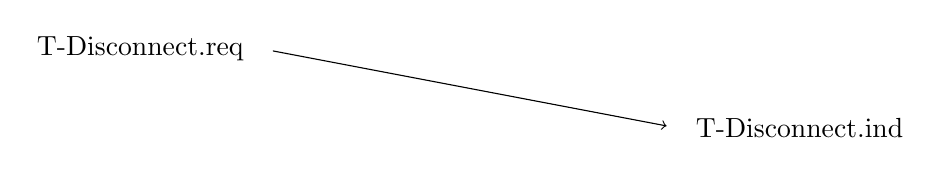
\begin{tikzpicture}[->]
		          	\tikzTimeDiagram{2}{2}
		          	
		          	\node[label = left:T-Disconnect.req, anchor = east] (a) at (5, -1) {};
		          	\node[label = right:T-Disconnect.ind, anchor = west] (b) at (10, -2) {};
		          	\draw (a) to (b);
	         	\end{tikzpicture}
	         	\caption{Verbindungsabbau durch Nutzer}
			\end{figure}
             
			\begin{figure}[H]
	        	\centering
	        	\begin{tikzpicture}[->]
		         	\tikzTimeDiagram{2}{1}
		         	
		         	\node[label = left:T-Disconnect.ind, anchor = east] (a) at (5, -1) {};
		         	\node[label = right:T-Disconnect.ind, anchor = west] (b) at (10, -1) {};
		         	\coordinate (center) at ($(a)!0.5!(b)$);
		         	\draw [bend left = 45] (a) to (center);
		         	\draw [bend left = 45] (b) to (center);
	        	\end{tikzpicture}
	        	\caption{Verbindungsabbau durch Provider}
			\end{figure}
			
			\begin{figure}[H]
				\centering
				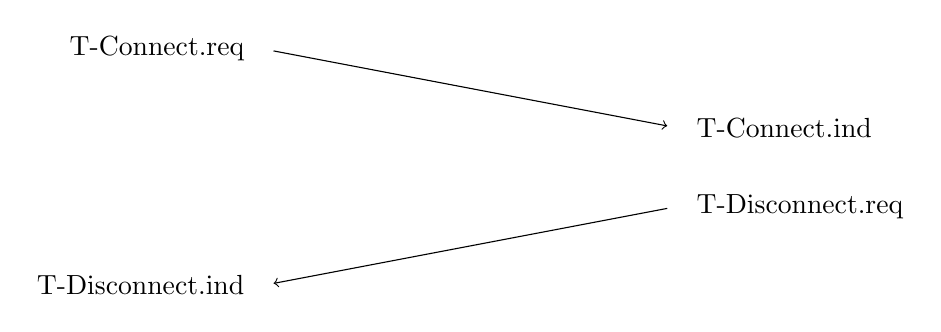
\begin{tikzpicture}[->]
					\tikzTimeDiagram{2}{4}
					
					\node[label = left:T-Connect.req, anchor = east] (a) at (5, -1) {};
					\node[label = right:T-Connect.ind, anchor = west] (b) at (10, -2) {};
					\node[label = right:T-Disconnect.req, anchor = west] (c) at (10, -3) {};
					\node[label = left:T-Disconnect.ind, anchor = east] (d) at (5, -4) {};
					\draw (a) to (b);
					\draw (c) to (d);
				\end{tikzpicture}
				\caption{Ablehnung des Verbindungsaufbaus}
			\end{figure}
			
			\begin{itemize}
				\item Die Verbindung wird regulär abgebaut.
				\item Dies kann zu einem Datenverlust führen, wenn die Verbindung zu früh abgebaut wird.
				\item Impliziter Abbau: Schließen des Sockets und nicht mehr antworten.
				\item Expliziter Abbau: Verbindungsfreigabe mittels \texttt{T-Disconnect}.
				\item \textbf{Problematik:} Es ist unmöglich sicherzustellen, dass keine Daten mehr unterwegs sind. \\ Sämtliche Pakete können verloren gehen, \dots, siehe \textit{Two Army Problem}
			\end{itemize}
        % end
        
        \subsection{Beispiellauf}
            \begin{figure}[H]
            	\centering
            	\begin{tikzpicture}[->]
	            	\tikzTimeDiagram{2}{12}
	            	
	            	\node[label = left:T-Connect.req, anchor = east] (a1) at (5, -1) {};
	            	\node[label = left:T-Connect.cnf, anchor = east] (a2) at (5, -4) {};
	            	\node[label = left:T-Data.req, anchor = east] (a3) at (5, -5) {};
	            	\node[label = left:T-Data.req, anchor = east] (a4) at (5, -7) {};
	            	\node[label = left:T-Data.ind, anchor = east] (a5) at (5, -9) {};
	            	\node[label = left:T-Disconnect.req, anchor = east] (a6) at (5, -11) {};
	            	
	            	\node[label = right:T-Connect.ind, anchor = west] (b1) at (10, -2) {};
	            	\node[label = right:T-Connect.rsp, anchor = west] (b2) at (10, -3) {};
	            	\node[label = right:T-Data.ind, anchor = west] (b3) at (10, -6) {};
	            	\node[label = right:T-Data.req, anchor = west] (b4) at (10, -8) {};
	            	\node[label = right:T-Data.ind, anchor = west] (b5) at (10, -10) {};
	            	\node[label = right:T-Disconnect.ind, anchor = west] (b6) at (10, -12) {};

	            	\draw (a1) to (b1);
	            	\draw (a3) to (b3);
	            	\draw (a4) to (b5);
	            	\draw (a6) to (b6);
	            	
	            	\draw (b2) to (a2);
	            	\draw (b4) to (a5);
            	\end{tikzpicture}
            	\caption{Ablehnung des Verbindungsaufbaus}
            \end{figure}
        % end
	% end

    \section{Verlässliche Zustellung}
        \begin{itemize}
        	\item Bisher werden Pakete so gut es geht zugestellt.
        	\item Allerdings können Pakete verloren gehen oder beschädigt werden (Bitfehler, Congestion, \dots)
        	\item Somit sollte der Sender darüber Informiert werden, dass etwas schief gelaufen ist \\ \(\rightarrow\) Sende für jedes Paket ein Acknowledge (ACK) \\ \(\rightarrow\) Weitere Probleme (hohes Datenaufkommen, \dots)
        	\item Was kann ein Sender tun, wenn ein Paket nicht bestätigt wurde?
	        	\begin{enumerate}
	        		\item Das Paket erneut senden.
	        		\item Die Datenrate reduzieren.
	        	\end{enumerate}
        \end{itemize}

        \subsection{Fehlersteuerung}
            \warning{Nicht alle Fehler können erkannt werden. Mit einer geringen Chance kann es bspw. passieren, dass sich sowohl Daten als auch Prüfsumme ändern.}
            
            \begin{itemize}
            	\item Wenn ein Fehler erkannt wird (Seiten des Empfängers), so wird das Paket meist einfach gedroppt.
            	\item In wenigen Fällen gibt der Empfänger dies auch über ein NACK (Negative ACK) bekannt (oftmals aber erst nach dem nächsten Paket, da sonst nicht geprüft werden könnte, dass ein Paket fehlt).
            \end{itemize}
        % end

        \subsection{Automatic Repeat reQuest (ARQ)}
            \begin{description}[leftmargin = 2cm]
            	\item[ARQ Typ 1] Stop-and-Wait ARQ
                	\begin{itemize}
                		\item Entspricht dem Alternating-Bit Protocol (\ref{sec:abp})
                		\item Schlechte Performanz bei schnellen oder breiten Netzwerken
                	\end{itemize}
            	\item[ARQ Typ 2] Go-Back-N ARQ
                	\begin{itemize}
                		\item Angenommen, das aktuelle und das nächste Paket gehen verloren \\ Bei alten Data Link Schichten kann der Empfangspuffer nur ein Element halten, d.h. out-of-order Pakete werden verworfen.
                		\item Wird ein verlorenes Paket erkannt, so werden alle vorherigen Pakete erneut gesendet (bis zum letzten ACK).
                		\item Bei einem Timeout wird nur das betroffene Paket erneut versendet.
                	\end{itemize}
            \end{description}
        % end
	% end

    \section{Flow Control}
        \begin{itemize}
        	\item \textbf{Aufgabe:} Schützen des Empfängers vor zu vielen eingehenden Paketen.
        	\item Link Layer: Schutz vor zu vielen weitergeleiteten Paketen.
        	\item Höhere Schichten (Network/Transport): Schutz vor zu vielen Verbindungen.
        	\item TCP implementiert Flow Control, dies ist auf Ebene 4 (Transport) aber kompliziert:
            	\begin{itemize}
            		\item Die Paketgröße ist sehr variabel.
            		\item Die Antwort von Prozessen kann sehr lange dauern.
            		\item Mit mehreren parallelen Verbindungen müssen dynamische Puffer alloziert werden, auf unteren Schichten würde eine fixe Größe ausreichen.
            	\end{itemize}
        \end{itemize}

        \subsection{Puffer Allokation}
            \begin{itemize}
            	\item Der Empfänger muss eingehende Pakete zwischenspeichern, bevor diese verarbeitet werden können.
            	\item Um dies zu unterstützen, muss der Sender:
                	\begin{itemize}
                		\item sich darauf verlassen, dass eingehende Pakete direkt bearbeitet werden (sehr unrealistisch!).
                		\item erwarten, dass genug Speicherplatz im Puffer verfügbar ist.
                	\end{itemize}
            \end{itemize}
            
            \textbf{Mögliche Implementierungen:}
            \begin{itemize}
            	\item Der Empfänger verlangsamt den Sender, wenn kein Speicher mehr verfügbar ist (implizit oder explizit).
            	\item Der Sender fragt einen bestimmten Pufferplatz an.
            	\item Der Empfänger teilt dem Sender mit, wie viel Platz er noch im Puffer hat (Beeinflussung der Datenrate oder \enquote{Credit} des Senders).
            \end{itemize}
        % end

        \subsection{Alternating-Bit Protocol}
            \label{sec:abp}
        
            \begin{itemize}
            	\item Der Sender wird bei jedem Paket informiert, wenn es eingetroffen ist (ACK).
            	\item Timeout beim Sender \\ \(\implies\) Paket verschwunden, ACK verschwunden, ACK verspätet \\ \(\implies\) Daten erneut senden.
            	\item Dies ist allerdings sehr langsam, da der Sender andauernd warten muss und annähernd durchgehend im Idle ist. Ebenso der Empfänger.
            \end{itemize}
        % end

        \subsection{Stop/Continue Nachrichten}
	        \begin{itemize}
	        	\item Es werden explizite Benachrichtigungen (\textit{Stop}, Continue) ausgetauscht als Flow Control.
	        	\item Wenn der Empfänger nicht mit den eingehenden Daten mithalten kann, sendet er ein \textit{Stop}.
	        	\item Nach Verarbeitung der Daten wird ein \textit{Continue} gesendet.
	        \end{itemize}
        % end

        \subsection{Rate Basiert}
            \begin{itemize}
            	\item Eine andere Methode für Flow Control.
            	\item Der Empfänger gibt an, welche Datenrate er maximal verarbeiten kann.
            	\item Der Sender hält sich an diese Datenrate und überflutet den Empfänger somit nicht.
            	\item Vorteile:
                	\begin{itemize}
                		\item Es werden wenig Nachrichten ausgetauscht \(\implies\) geringer Overhead.
                		\item Netzwerk und Empfänger werden \enquote{sanft} ausgelastet, es gibt keine einzelnen hohen Spikes.
                	\end{itemize}
                \item Nachteile:
	                \begin{itemize}
	                	\item Es werden keine Informationen über erfolgreichen Datenempfang gesendet. \\ \(\implies\) Ergibt keinen Sinn für verlässlichen Transport über unzuverlässige Netze. \\ \(\implies\) Es muss eine separate ACK/Repeat Methode geben. \\ \(\implies\) Dies kann die Erwartung der Datenrate stören.
	                \end{itemize}
            \end{itemize}
        % end

        \subsection{Credit Basiert}
            \begin{itemize}
            	\item Der Empfänger teilt dem Sender regelmäßige \textit{Credits} zu, sodass dieser senden darf.
            	\item Der Sender stoppt die Übertragung, wenn er keine Credits mehr hat.
            	\item Explizites Fehlerkontrolle ist nötig, um Fehler zu erkennen.
            \end{itemize}
            
            \subsubsection{Absolute Credits}
                \begin{itemize}
                	\item Der Empfänger weißt dem Sender eine absolute Anzahl Credits zu.
                \end{itemize}
            % end

            \subsubsection{Sliding Window}
                \begin{itemize}
                	\item Credits werden in Relation zu den ankommenden ACKs vergeben.
                \end{itemize}
			% end
        % end
	% end

    \section{Congestion Control}
        \begin{itemize}
        	\item In Netzwerken kann es zu Verstopfung (Congestion) kommen, da die Elemente eine begrenzte Bandbreite haben.
        	\item Werden mehr Daten in das Netzwerk gegeben als verarbeitbar sind, so bricht das Netzwerk zusammen (\textit{Congestion Collapse}) und es gehen Pakete verloren.
        	\item Gehen Pakete verloren (bspw. durch volle Puffer), so sind die verbrauchten Netzwerkressourcen verschwendet worden.
            	\begin{itemize}
            		\item Dies führt zu einem Schneeball-Effekt, da das Netzwerk mit neu gesendeten Paketen (aufgrund von Verlust) geflutet wird.
            		\item Dies führt wieder zu mehr Traffic.
            		\item Mehr Pakete gehen verloren.
            		\item \dots
            	\end{itemize}
            \item \textbf{Lösung:} Die Senderate muss an das Netzwerk angepasst werden. \\ Dies hängt von allen Komponenten im Netzwerk ab und ist damit sehr komplex.
        \end{itemize}
        
        \paragraph{Abgrenzung Flow Control \( \leftrightarrow \) Congestion Control}
            \textit{Flow Control} beschäftigt sich damit, dass \textit{einzelne Knoten} nicht überlaufen, \\
            \indent \textit{Congestion Control} beschäftigt sich damit, dass das \textit{gesamte Netzwerk} nicht überläuft.
        % end

        \subsection{Design Properties/Options}
            \begin{description}
            	\item[Fairness] Das System sollte Fair sein, d.h. jeder Knoten sollte fair viele Ressourcen zur Verfügung haben. \\ Dies heißt nicht, dass jeder Knoten gleich viele Ressourcen braucht (Bsp.: Telnet vs. Videokonferenz).
            	\item[Router-Basiert vs. Host-Basiert] Wo werden die Informationen gesammelt, Entscheidungen getroffen, Aktionen angewandt?
            	\item[Window-Basiert vs. Rate-Basiert] Wie wird beschrieben, wie viel Traffic ein Host in das Netzwerk senden darf?
                	\begin{itemize}
                		\item Rate - Eine bestimmte Anzahl Bytes pro Sekunde
                		\item Congestion Window - Eine Anzahl Bytes, die gesendet werden darf, bevor neue Credits vergeben werden.
                	\end{itemize}
            	\item[Open Loop] Das System ist so gestaltet, dass es von vornherein funktioniert und zur Laufzeit keine Anpassungen notwendig sind.
            	\item[Closed Loop] Das System nutzt eine Art Feedback, um sich den Gegebenheiten anzupassen.
            	\item[Implizites Feedback] Congestion wird von dem Sender erkannt (bspw. durch ausbleibende ACKs).
            	\item[Explizites Feedback] Congestion informiert den Sender (auf irgendeine Art).
            \end{description}
        % end

        \subsection{Pakete Verwerfen, Implizites Feedback, Mögliche Aktionen}
            \textit{Sei ein Router gegeben, dessen Puffer vollgelaufen ist.}
        
            \begin{itemize}
            	\item Welches Paket soll verworfen werden, wenn ein neues eintrifft?
            	\item \textbf{Drop Tail:} Das neuste Paket (welches am Ende einsortiert wird) wird verworfen. \\ Annahme: Alte Pakete sind wichtiger als neue.
            	\item \textbf{Drop Any:} Um das neue Paket einfügen zu können, wird ein Paket verworfen, welches schon länger in der Warteschlange wartet. \\ Annahme: Neue Pakete sind wichtiger als alte (bspw. bei Livestreams).
            \end{itemize}
            
            \paragraph{Feedback}
	            \begin{itemize}
	            	\item Der Verwurf eines Paketes stellt \textit{implizites Feedback} dar, da das Paket verloren geht. Dies kann bspw. durch fehlende ACKs vernommen werden.
		            \item Unter der Annahme, das Pakete nur verloren gehen, wenn Congestion auftritt, sollte der Sender seine Senderate verringern. \\ In Kabelgebundenen Netzen mag dies zutreffen, nicht aber bei WLAN-Netzen.
	            \end{itemize}
	            
	            \warning{In Open Loop Systemen sollte eine voller Puffer nie auftreten, da sonst das System nicht korrekt gestaltet ist.}
            % end
            
            \paragraph{Erhalt von Feedback}
	            \textit{Ein Sender hat (auf irgendeine Weise) mitbekommen, dass Congestion aufgetreten ist.}
            
	            \begin{itemize}
	            	\item Bei \textbf{Rate Basierten} Systemen sollte der Sender seine Senderate reduzieren.
	            	\item Bei \textbf{Window Basierten} System sollte der Sender sein Window verkleinern.
	            \end{itemize}
	            
	            Dies wird bei TCP näher betrachtet (\ref{sec:tcpcongestioncontrol}).
            % end
        % end

        \subsection{Proaktive Aktionen}
            \begin{itemize}
            	\item Da Congestion nicht gut ist, sollte dies möglichst früh vermieden werden.
            	\item Hierzu sind \textit{proaktive Aktionen} sinnvoll, durch die Sender frühzeitig Informiert werden, wenn ein Puffer volllaufen sollte (o.ä.).
            	\item Ein solcher Zustand im Router wird \textit{Warning State} genannt.
            \end{itemize}

            \subsubsection{Choke Pakete}
                \begin{itemize}
                	\item Stellt ein Router fest, dass er congested ist oder dies bald sein wird, so sendet dieser \textit{Choke Pakete}.
                	\item Ein Choke Paket teilt dem Sender mit, dass dieser seine Senderate reduzieren sollte.
                	\item \textbf{Problematik:} In einem bereits verstopften Netzwerk können Choke Pakete zu noch mehr Congestion führen.
                	\item \textbf{Problematik 2:} Es kann lange dauern, bis der Sender merkt, dass Choke Pakete gesendet wurden.
                \end{itemize}
			% end

            \subsubsection{Warning Bits}
                \begin{itemize}
                	\item Stellt ein Router fest, dass er congested ist oder dies bald sein wird, so setzt dieser ein \textit{Warning Bit} in allen Paketen, die ausgesendet werden.
                	\item Das Ziel kopiert dieses Bit in das ACK-Paket.
                	\item Der Sender empfängt das Bit und reduziert seine Senderate.
                \end{itemize}
			% end

            \subsubsection{Random Early Detection (RED)}
                \begin{itemize}
                	\item Verlorene Pakete werden als implizites Feedback gewertet.
                	\item Es werden Pakete verworfen, selbst wenn der Puffer noch nicht voll ist.
                	\item Ein eingehendes Paket wird mit einer gewissen Wahrscheinlichkeit verworfen, die bis zu einem gewissen Punkt mit der Anzahl Elemente im Puffer steigt.
                \end{itemize}
			% end
        % end
	% end

    \section{UDP}
        Das \textit{User Datagram Protocol} (UDP) ist verbindungslos, stateless, hat kein Congestion Control und keine Empfangsbestätigung. Die Pakete kommen nach bester Möglichkeit an, können aber verloren gehen. Dies ist für Multi-Media Anwendungen sinnvoll, bei denen Echtzeit wichtiger ist als Vollständigkeit (bspw. VoIP).
        
        Dadurch ist UDP sehr einfach, es stellt sich allerdings die Frage, weshalb nicht einfach IP gesprochen wird? Der Grund liegt darin, dass UDP Multiplexing (Ports) unterstützt und somit mehrere Prozesse auf einem Host UDP sprechen können.

        \subsection{Datagramm-Format}
            \begin{figure}[H]
            	\centering
            	\begin{bytefield}[bitwidth = 1.2em]{32}
            		\bitheader{0-31} \\
            		\begin{rightwordgroup}{Header}
            			\bitbox{16}{Source Port} & \bitbox{16}{Destination Port} \\
            			\bitbox{16}{Length} & \bitbox{16}{Checksum}
            		\end{rightwordgroup} \\
            		\begin{rightwordgroup}{Body}
	            		\bitbox[trl]{32}{} \\
	            		\bitbox[rl]{32}{Data} \\
	            		\bitbox[rbl]{32}{} \\
            		\end{rightwordgroup}
            	\end{bytefield}
            	\caption{UDP Paketformat}
            	\label{fig:udppacket}
            \end{figure}
            
            \begin{description}
            	\item[Source Port] 16 Bit breit. Der Quellport.
            	\item[Destination Port] 16 Bit breit. Der Zielport.
            	\item[Length] 16 Bit breit. Die Gesamtlänge des Datagramms in Byte. Somit kann ein Datagramm maximal \( 2 ^ 16 - 1 = 65535\text{ Byte} \) lang sein.
            	\item[Checksum] 16 Bit breit. Die Prüfsumme über die Kopfdaten. Zur Berechnung wird das Feld auf 0 gesetzt und der Header in 16 Bit Worte unterteilt. Für die weitere Berechnung siehe \ref{sec:checksumonescomplement}.
            	\item[Data] Die Nutzdaten des Datagramms.
            \end{description}
        % end

        \subsection{Demultiplexing} % 4.70, 4.71
            Siehe \ref{sec:demultiplexing}.
        % end
	% end

    \section{TCP}
        Das \textit{Transport Control Protocol} (TCP) ist das Standard Protokoll im Internet und annähernd jedes andere Protokoll setzt auf TCP auf.
        
        TCP implementiert die folgenden Features:
        \begin{itemize}
        	\item Punkt-zu-Punkt \\ Pro Verbindung gibt es einen Sender und einen Empfänger.
        	\item Verlässlich und in-Order \\ Alle Pakete kommen gesichert und in der richtigen Reihenfolge an oder es wird über einen Verlust berichtet.
        	\item Vollduplex \\ Daten können in beide Richtungen gesendet werden.
        	\item Sende- und Empfangspuffer
        	\item Verbindungsorientiert \\ Handshaking (Drei-Wege Handschlag) initialisiert Sender und Empfänger bevor Daten gesendet werden können.
        	\item Flow Control \\ Der Sender kann den Empfänger nicht überlasten.
        	\item Congestion Control \\ Der Sender passt das Congestion Window an und übernimmt neue Senderaten.
        \end{itemize}

        \subsection{Paket-Format}
            \begin{figure}[H]
            	\centering
            	\begin{bytefield}[bitwidth = 1.2em]{32}
            		\bitheader{0-31} \\
            		\begin{rightwordgroup}{Header}
	            		\bitbox{16}{Source Port} & \bitbox{16}{Destination Port} \\
	            		\bitbox{32}{Sequence Number} \\
	            		\bitbox{32}{Acknowledge Number} \\
	            		\bitbox{4}{Header Length} & \bitbox{4}{Reserved} &
	            		\bitbox{8}{Flags} & \bitbox{16}{Window} \\
	            		\bitbox{16}{Checksum} & \bitbox{16}{Urgent Pointer} \\
			            \bitbox{26}{Options \textit{(optional)}} & \bitbox{6}{Padding}
            		\end{rightwordgroup} \\
            		\begin{rightwordgroup}{Body}
            			\bitbox[trl]{32}{} \\
            			\bitbox[rl]{32}{Data} \\
            			\bitbox[rbl]{32}{} \\
            		\end{rightwordgroup}
            	\end{bytefield}
            	\caption{TCP Paketformat}
            	\label{fig:tcppacket}
            \end{figure}
            
            \begin{description}
            	\item[Source Port] 16 Bit breit. Der Quellport.
            	\item[Destination Port] 16 Bit breit. Der Zielport.
            	\item[Sequence Number] 32 Bit breit. Die Sequenznummer des Pakets.
            	\item[Acknowledge Number] 32 Bit breit. Die Sequenznummer des Paketes, welches bestätigt wird (plus die Länge des bestätigten Paketes).
            	\item[Header Length] 4 Bit breit. Die Länge der Kopfdaten in 32 Bit Worten.
            	\item[Flags] 6 Bit breit. Schalter zur Steuerung von bspw. dem Verbindungsaufbau in der folgenden Reihenfolge:
	            	\begin{itemize}
	            		\item[\textbf{URG}] Urgent - Markiert alle Daten bis zu dem Byte Feld, auf das der \textit{Urgend Pointer} zeigt, als dringend. Der Empfänger soll diese Daten bevorzugt behandeln. In der Regel wird das Feld aber nicht ausgewertet.
	            		\item[\textbf{ACK}] Acknowledge - Zeigt an, dass das \textit{Acknowledge}-Feld gültig ist und ein Paket bestätigt wird.
	            		\item[\textbf{PSH}] Push - Weißt den Empfänger an, sowohl Eingangs- als auch Ausgangspuffer zu umgehen. In der Regel tut das Feld aber etwas anderes.
	            		\item[\textbf{RST}] Reset - Bricht die Verbindung ab.
	            		\item[\textbf{SYN}] Synchronize - Initiiert eine neue Verbindung. Der Server sollte mit \textit{SYN}+\textit{ACK} antworten, oder mit \textit{RST}.
	            		\item[\textbf{FIN}] Finish - Gibt die Verbindung frei und zeigt an, dass keine weiteren Daten kommen werden.
	            	\end{itemize}
            	\item[Window] 16 Bit breit. Die Anzahl an Bytes, die der Sender dieses Pakets bereit ist zu Empfangen. Dient Flow Control.
            	\item[Checksum] 16 Bit breit. Die Prüfsumme über die Kopfdaten. Zur Berechnung wird das Feld auf 0 gesetzt und der Header in 16 Bit Worte unterteilt. Für die weitere Berechnung siehe \ref{sec:checksumonescomplement}.
            	\item[Urgent Pointer] 16 Bit breit. Zeigt, in Kombination mit dem Schalter \textit{URG}, auf das erste nicht-dringende Byte in den Daten.
	        	\item[Options and Padding \textit{(optional)}] 0 bis 40 Byte breit. Bis zu 40 Byte an Optionen, wobei verbleibende Bytes bis zum nächsten 32 Bit Wort mit Nullen aufgefüllt werden (Padding).
            	\item[Data] Die Nutzdaten des Paketes.
            \end{description}
        % end

        \subsection{Demultiplexing}
            Siehe \ref{sec:demultiplexing}.
            
            In TCP wird ein \textit{Socket} durch ein 4-Tupel (Quell IP, Quell Port, Ziel IP, Ziel Port) identifiziert. Ein Host nutzt alle vier Teile, um ein Paket dem korrekten Prozess zuzuordnen. Ein Server kann viele Sockets gleichzeitig unterstützen, jeder mit einem eigenen 4-Tupel.
        % end

        \subsection{Sequenznummern, ACKs}
            Die Sequenznummern werden wie folgt vergeben:
            \begin{itemize}
            	\item Jedes Paket enthält die bis dahin versendeten Bytes.
            	\item Damit ist es für den Empfänger möglich zu prüfen, ob alle Bytes erhalten wurden.
            \end{itemize}
            Die ACK-Nummern werden wie folgt vergeben:
            \begin{itemize}
            	\item Jedes ACK-Paket enthält die bis dahin empfangenen Bytes. Vorherige ACKs werden nicht erneut gesendet.
            	\item Damit ist es für den Sender möglich zu prüfen, ob alle Bytes angekommen sind.
            	\item Ein ACK kann entweder \enquote{huckepack} mit einem Datenpaket versendet werden oder einzeln.
            \end{itemize}
            
            \paragraph{Beispiel}
                \begin{figure}[H]
                	\centering
                	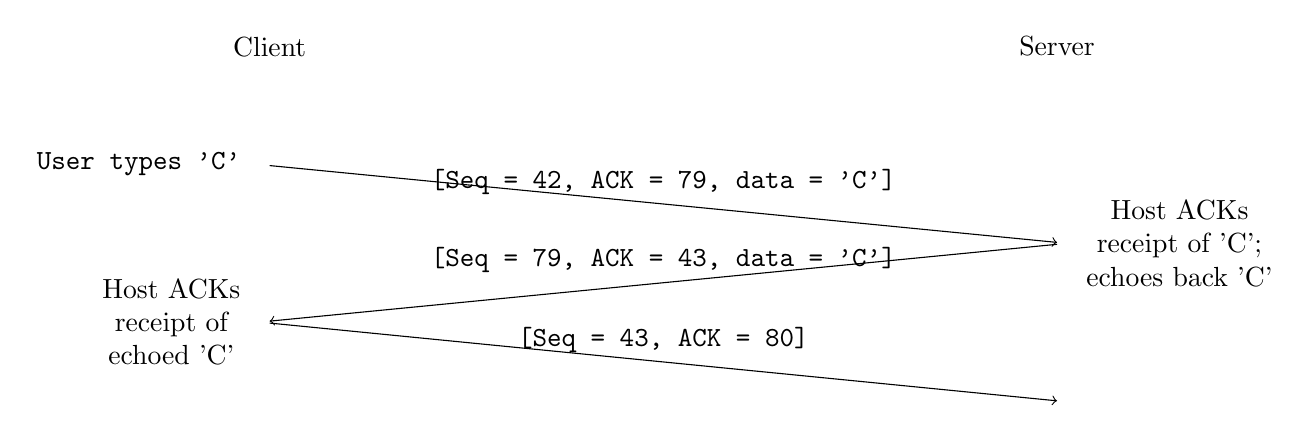
\begin{tikzpicture}[align = center]
	                	\tikzTimeDiagram[2]{2}{4}
	                	
	                	\node [label = left:\texttt{User types 'C'}, anchor = east] (a) at (10, -1) {};
	                	\node [label = right:{Host ACKs\\receipt of 'C';\\echoes back 'C'}, anchor = west] (b) at (20, -2) {};
	                	\node [label = left:{Host ACKs\\receipt of\\echoed 'C'}, anchor = east] (c) at (10, -3) {};
	                	\coordinate (d) at (20, -4);
	                	
	                	\node at (10, 0.5) {Client};
	                	\node at (20, 0.5) {Server};
	                	
	                	\draw [->] (a) to node[above]{\texttt{[Seq = 42, ACK = 79, data = 'C']}} (b);
	                	\draw [->] (b) to node[above]{\texttt{[Seq = 79, ACK = 43, data = 'C']}} (c);
	                	\draw [->] (c) to node[above]{\texttt{[Seq = 43, ACK = 80]}} (d);
                	\end{tikzpicture}
                	\caption{TCP: Sequenznummern + ACK; Szenario: Telnet}
                \end{figure}
            % end

            \subsubsection{Retransmission}
                Der Sender überträgt ein Paket erneut, falls:
                \begin{itemize}
                	\item Timeout: Ein ACK nicht innerhalb einer erwarteten Zeit eingetroffen ist (sende nur das Paket, dessen ACK fehlt erneut).
                \end{itemize}
                Der Empfänger überträgt ein ACK erneut, falls:
                \begin{itemize}
                	\item Nach einem gesendeten ACK ein Paket eintrifft, dessen Sequenznummer kleiner ist als die zuletzt gesendete ACK-Nummer, wird das höchstmögliche ACK erneut gesendet.
                \end{itemize}

                \paragraph{Fast Retransmit}
                    \begin{itemize}
                    	\item Die Timeout Zeit ist schwer \enquote{gut} zu wählen, denn:
	                    	\begin{itemize}
	                    		\item eine lange Zeit führt zu Verzögerungen und
	                    		\item eine kurze Zeit führt zu viel Traffic.
	                    	\end{itemize}
	                    \item Verlorene Pakete können mit duplizierten ACKs erkannt werden.
		                    \begin{itemize}
		                    	\item Wenn ein Paket verloren wird, werden viele duplizierte ACKs versendet.
		                    \end{itemize}
		                \item[\(\rightarrow\)] Wenn der Sender 3 ACKs für die selben Daten empfangen hat, wird davon ausgegangen, dass \textit{alle} Segmente seit diesen Daten verloren gegangen sind \(\rightarrow\) Alle Pakete erneut senden, bevor ein Timeout stattfindet.
                    \end{itemize}
                % end
            % end
        % end

        \subsection{Verbindungssteuerung}
            Verbindungen mit TCP können auf zwei Arten aufgebaut werden:
            \begin{description}
            	\item[Aktiv] Ein Prozess fragt explizit eine TCP-Verbindung an.
            	\item[Passiv] Ein Prozess informiert TCP, dass die Verbindungen annehmen kann.
                	\begin{itemize}
                		\item Dies kann ein spezifischer Socket sein oder
                		\item alle eingehenden Verbindungen werden angenommen (Beispiel: Web Server). \\ Sobald eine Anfrage eingeht, wird ein Socket erstellt.
                	\end{itemize}
            \end{description}
            
            \info{Applikationen wissen nicht, ob eine TCP Verbindung aufgebaut wurde. TCP implementiert die primitive \texttt{T-Connect.rsp} nicht.}
            
            \paragraph{Verbindungsphasen}
                \begin{itemize}
                	\item Verbindungsaufbau
	                	\begin{itemize}
	                		\item Drei-Wege Handschlag
	                		\item Einigung auf Window Size und Sequenznummern
	                	\end{itemize}
                	\item Datentransfer
	                	\begin{itemize}
		                	\item ACKs \enquote{huckepack} auf Datenpaketen
	                	\end{itemize}
                	\item Verbindungsabbau
	                	\begin{itemize}
	                		\item Bestätigt!
	                		\item Dies verhindert den Verlust bereits gesendeter Daten
	                	\end{itemize}
                \end{itemize}
                
                \begin{figure}[H]
                	\centering
                	\begin{tikzpicture}[->]
	                	\tikzTimeDiagram[2]{2}{18};
	                	
	                	\coordinate (a) at (10, -1);
	                	\coordinate (b) at (20, -2);
	                	\coordinate (c) at (20, -3);
	                	\coordinate (d) at (10, -4);
	                	\coordinate (e) at (10, -5);
	                	\coordinate (f) at (20, -6);
	                	
	                	\coordinate (g) at (10, -7);
	                	\coordinate (h) at (20, -8);
	                	\coordinate (i) at (20, -9);
	                	\coordinate (j) at (10, -10);
	                	
	                	\coordinate (k) at (10, -11);
	                	\coordinate (l) at (20, -12);
	                	\coordinate (m) at (20, -13);
	                	\coordinate (n) at (10, -14);
	                	\coordinate (o) at (20, -15);
	                	\coordinate (p) at (10, -16);
	                	\coordinate (q) at (10, -17);
	                	\coordinate (r) at (20, -18);
	                	
	                	\node at (10, 0.5) {Client};
	                	\node at (20, 0.5) {Server};
	                	
	                	\draw (a) to node[above]{\texttt{[SYN, seq = 17]}} (b);
	                	\draw (c) to node[above]{\texttt{[SYN, seq = 39, ACK = 18]}} (d);
	                	\draw (e) to node[above]{\texttt{[seq = 18, ACK = 40]}} (f);
	                	
	                	\draw (g) to node[above]{\texttt{[seq = 53, ACK = 78, data = 'hi']}} (h);
	                	\draw (i) to node[above]{\texttt{[seq = 78, ACK = 55, data = 'ho']}} (j);
	                	
	                	\draw (k) to node[above]{\texttt{[FIN]}} (l);
	                	\draw (m) to node[above]{\texttt{[ACK]}} (n);
	                	\draw (o) to node[above]{\texttt{[FIN]}} (p);
	                	\draw (q) to node[above]{\texttt{[ACK]}} (r);
                	\end{tikzpicture}
                	\caption{TCP Verbindungsphasen}
                \end{figure}
            % end
        % end

        \subsection{Senden/Empfangen Puffer}
            TCP hält einen Puffer vor für:
            \begin{itemize}
            	\item Ausgehende Pakete, um Fehlerkontrolle zu dienen.
            	\item Eingehende Pakete, die noch nicht verarbeitet wurden oder out-of-order empfangen wurden.
            \end{itemize}
        % end

        \subsection{Flow Control: Advertised Window}
            \begin{itemize}
            	\item In TCP teilt der Empfänger mit, wie viel Platz er im Empfangspuffer hat.
                	\begin{itemize}
                		\item Position des nächsten erwarteten Bytes: \textit{NextByteExpected}
                		\item Position des zuletzt gelesenen Bytes: \textit{LastByteRead}
                		\item Platz im Puffer: \( (\textit{NextByteExpected} - 1) - \textit{LastByteRead} \)
                		\item Maximaler Pufferspeicherplatz: \textit{MaxRecvdBuffer}
                		\item Ausgeschriebenes Pufferfenster: \( \textit{MaxRcvdBuffer} - ((NextByteExpected - 1) - LastByteRead) \)
                	\end{itemize}
                \item Das ausgeschriebene Pufferfenster (\textit{Advertised Window}) limitiert die Anzahl Daten, die der Sender schicken wird.
	                \begin{itemize}
	                	\item Der TCP Sender sorgt dafür, dass gilt: \( \textit{LastByteSent} - \textit{LastByteAcked} \leq \textit{AdvertisedWindow} \)
	                	\item[\(\iff\)] \( \textit{EffectiveWindow} = \textit{AdvertisedWindow} - (\textit{LastByteSend} - \textit{LastByteAcked}) \)
	                \end{itemize}
            \end{itemize}
            
            \subsubsection{Nagle-Algorithmus (Self-Clocking)}
                \begin{itemize}
                	\item Das Eintreffen eines ACKs is ein Indikator dafür, dass neue Daten gesendet werden können.
                	\item Trifft ein ACK für ein kleines Paket ein und es würde direkt ein neues, kleines, Paket versendet werden, würde das Netzwerk mit kleinen Paketen überlastet werden (\enquote{silly window syndrome}).
                	\item Dies wird durch den Nagle-Algorithmus verhindert.
                \end{itemize}
                
                \paragraph{Nagle-Algorithmus}
	                \begin{figure}[H]
	                	\centering
	                	\begin{lstlisting}
when (Application produces Data) {
	if (AvailableData >= MaxSegmentSize && AdvertisedWindow >= MSS) {
		send full segment
	} else if (UnACKed Data in flight) {
		buffer data
	} else {
		send segment
	}
}
	                	\end{lstlisting}
	                	\caption{Nagle-Algorithmus}
	                \end{figure}
	            % end
            % end
        % end

        \subsection{Congestion Control}
            \label{sec:tcpcongestioncontrol}
        
            \begin{itemize}
            	\item TCP nutzt implizites Feedback (bspw. durch den RED-Algorithmus) für Congestion Control.
            	\item Es existieren einige Vorschläge für explizites Feedback, diese sind aber nicht Teil des TCP-Standards.
            	\item Erwartung: Congestion ist der einzige wichtige GRund für verlorene Pakete.
            	\item TCP nutzt ein Window Basiertes Verfahren für Congestion Control.
                	\begin{itemize}
                		\item Der Sender passt auf, dass nicht mehr Daten als möglich versendet werden.
                		\item Es werden nur Daten gesendet, wenn \( \textit{LastByteSent} - \textit{LastByteAcked} \leq \textit{CongestionWindow} \) gilt.
                	\end{itemize}
            \end{itemize}

            \subsubsection{ACK-Clocking}
                \textit{Annahme: TCP hat auf irgendeine Weise die korrekte Größe des Congestion Windows bekommen. Außerdem wurde bereits die maximale Anzahl Daten versendet.}
                
                \begin{itemize}
                	\item Neue Daten dürfen gesendet werden, wenn:
                    	\begin{itemize}
                    		\item das Netzwerk wieder genug freie Ressourcen hat.
                    		\item Dies ist der Fall, wenn andere Pakete das Netzwerk verlassen haben.
                    		\item Durch eingehende ACKs wird der Sender hierüber informiert.
                    	\end{itemize}
                    \item Somit dient ein ACK nicht nur der Empfangsbestätigung, sondern auch der Erlaubnis, neue Pakete zu senden.
                    \item Gute Nachricht: Eintreffendes ACK \( \rightarrow \) Congestion Window vergrößern.
                    \item Schlechte Nachricht: Kein ACK, Timeout \( \rightarrow \) Congestion Window verkleinern.
                \end{itemize}
            % end

            \subsubsection{Additive/Multiplikative Erhöhung/Verringerung}
                Da ein überlastetes Netzwerk sehr schlecht ist, muss darauf schnell reagiert werden. Außerdem sollte bei guten Übertragungen die Rate erhöht werden, damit sich das Verfahren auf eine gute Rate einpendeln kann.
                
                Dies kann \textit{multiplikativ} (die Last um 50\% reduzieren) oder \textit{additiv} (die Last um einen bestimmten Wert erhöht) stattfinden.
                
                Folgende Kombinationen für Erhöhung/Verringerung wären möglich:
                \begin{description}
                	\item[AIAD] Additive Increase, Additive Decrease
                    	\begin{itemize}
                    		\item Reagiert nicht schnell genug auf Congestion im Netzwerk.
                    	\end{itemize}
                	\item[AIMD] Additive Increase, Multiplicative Decrease
                    	\begin{itemize}
                    		\item Reagiert schnell auf Congestion und
                    		\item Erhöht die Senderate moderat.
                    		\item Somit ist \textbf{AIMD} die einzige gute Option!
                    	\end{itemize}
                	\item[MIAD] Multiplicative Increase, Additive Decrease
                    	\begin{itemize}
                    		\item Reagiert nicht schnell genug auf Congestion im Netzwerk.
                    	\end{itemize}
                	\item[MIAM] Multiplicative Increase, Multiplicative Decrease
                    	\begin{itemize}
                    		\item Reagiert schnell auf Congestion, aber:
                    		\item Überlastet das Netzwerk sehr schnell, da mit MI schnell über das Ziel hinaus geschossen wird.
                    	\end{itemize}
                \end{description}
                
                Additive Increase erhöht das Congestion Window wie folgt:
                \begin{align*}
                	\text{Increment}         & = \text{MSS} \cdot \frac{\text{MSS}}{\text{Congestion Window}} \\
                	\text{Congestion Window} & = \text{Congestion Window} + \text{Increment}
                \end{align*}
                
                Allerdings kann TCP hiermit schnell überreagieren, wenn Pakete aus anderen Gründen nicht ankommen (bspw. Verbindungsfehler). In Kabelnetzen passiert dies selten, kann aber zu großen Problem führen in Kabellosen Netzen.
            % end

            \subsubsection{Slow Start}
                \textit{Slow Start} ist eine Methode, um TCP Verbindungen schnell auf ein vernünftiges Congestion Window zu heben, da dies mit AI sehr lange dauert.
                
                \begin{itemize}
                	\item In der \textit{Slow Start Phase} wird das Congestion Window bei jedem eintreffenden ACK verdoppelt.
                	\item Geht auch nur ein ACK verloren (das Netzwerk ist überlastet), geht TCP in die \textit{Congestion Avoidance Phase} über. \\ Diese entspricht dem normalen TCP Congestion Control mit AIMD.
                \end{itemize}
            % end
            
            \subsubsection{Zusammenfassung Congestion Control}
                \begin{itemize}
                	\item Ist das Congestion Window kleiner als ein bestimmter Threshold (Congestion) und der Sender ist in der Slow Start Phase, so wächst das Window exponentiell.
                	\item Ist das Congestion Window größer als ein bestimmter Threshold (Congestion), wechselt der Sender in die Congestion Avoidance Phase und das Window wächst linear.
                	\item Tritt ein dreifaches ACK auf, so wird der Threshold auf die Hälfte des Congestion Window gesetzt und das Congestion Window wird auf den Threshold gesetzt (das Window wird halbiert).
                	\item Tritt ein Timeout auf, so wird der Threshold auf die Hälfte des Congestion Window gesetzt und das Congestion wird auf eine MSS gesetzt.
                \end{itemize}
            % end
        % end
	% end

    \section{Stream Control Transmission Protocol (SCTP)}
        Das \textit{Stream Control Transmission Protocol} (SCTP) ist:
        \begin{itemize}
        	\item Nachrichten-Orientiert (wie UDP), bietet aber Flow Control, Congestion Control, Fehlerkontrolle und
        	\item stellt die Zustellung und die korrekte Reihenfolge von Nachrichten sicher.
        \end{itemize}
        
        Bisher ist SCTP noch nicht in Betriebssystemen verfügbar, es existieren aber Libraries für den Userspace.
        
        \textbf{Features:}
        \begin{itemize}
        	\item Flexible Nachrichten-Orientierte Streams
            	\begin{itemize}
            		\item Jeder Nachricht in einem Stream wird eine Sequenznummer zugewiesen, um die Reihenfolge sicherzustellen.
            		\item Der Empfänger kann Sortierung und Zustellungssicherung aktivieren/deaktivieren.
            		\item Der Sender kann Fragmentierung und Nagle aktivieren/deaktivieren.
            	\end{itemize}
            \item Multi-Streaming: Mehrere unabhängige Streams können mittels Multiplexing über eine Verbindung gesendet werden.
	            \begin{itemize}
	            	\item Unabhängige Sortierung.
	            	\item Ein Browser kann bspw. Text in einem Stream und Bilder in einem anderen versenden.
	            \end{itemize}
		    \item Multi-Homing: Sowohl Sender als auch Empfänger können beide mehrere IP Adressen haben.
        \end{itemize}
	% end

    \section{Datagram Congestion Control Protocol (DCCP)}
        Das \textit{Datagram Congestion Control Protocol} (DCCP) ist:
        \begin{itemize}
        	\item für Applikationen, welche unzuverlässige, schnelle Übertragung benötigen wobei
        	\item Congestion Control benötigt wird, was DCCP bietet.
        \end{itemize}
        
        Im Grunde ist DCCP:
        \begin{itemize}
        	\item TCP ohne Streams und Verlässlichkeit oder
        	\item UDP mit Congestion Control, Handshakes und ACKs (optional).
        \end{itemize}
        
        \textbf{Features:}
        \begin{itemize}
        	\item Unzuverlässiger Nachrichtentransport
        	\item Separate Header/Data Prüfsummen
        	\item Nachrichten-Orientiert
        	\item Verlässliche ACKs für Congestion Control
        	\item Multi-Homing wie bei SCTP
        \end{itemize}
	% end

    \section{Realtime Transfer (Control) Protocol (RTP/RTCP)}
        Das \textit{Realtime Transfer Protocol} (RTP) ist:
        \begin{itemize}
        	\item primär als Multimedia Protokoll gedacht, da es
        	\item sehr gut auf große Netzwerke skaliert.
        \end{itemize}
        
        \textbf{Features:}
        \begin{itemize}
        	\item Sequenznummern und Zeitstempel
        	\item Eindeutige Quell/Sitzungs-ID (SSRC oder CSRC)
        	\item Verschlüsselung
        	\item Codec
        \end{itemize}
        
        Die Daten werden dabei über RTP versendet und die Kontrolle findet über das \textit{Realtime Transfer Control Protocol} (RTCP) statt.
        
        RTP baut auf UDP auf, somit gibt es außerdem alle Features von UDP:
        \begin{itemize}
        	\item Ports, IP Adressen
        	\item Paketnummerierung,
        	\item \dots
        \end{itemize}
	% end

    \section{QUIC}
        \textit{Quick UDP Internet Connections} (QUIC) ist ein von Google vorgestelltes Protokoll, welches aktuell in einem Standardisierungsprozess beim der IETF ist.
        
        QUIC unterstützt sehr effiziente Verschlüsselung bei geringer Latenz und baut auf UDP auf.
        
        Protokolle, welche auf UDP aufbauen haben den Vorteil, dass Firewalls mit diesen arbeiten können und keine speziellen Regeln gebaut werden müssen.
        
        Da Verschlüsselung schnell ausgetauscht werden muss (z.B. bei Security-Updates), läuft QUIC im Userspace eines Systems und nicht im Kernel, wodurch nicht das OS geupdated werden muss, um QUIC zu updaten.
	% end
% end

\chapter{Warteschlangentheorie}
    Die Warteschlangentheorie beschäftigt sich mit folgenden Themen in einem Warteschlangen/Server-System (ein Server arbeitet die Anfragen ab):
    \begin{enumerate}
    	\item \textit{Ankunft} Wie viele Anfragen treffen ein? \\ Üblicherweise als \textit{Wahrscheinlichkeitsverteilung über Zeitintervalle} angegeben
    	\item \textit{Service} Wie lange dauert es, Anfragen zu bearbeiten? \\ Servicezeit, Wahrscheinlichkeit von einer Bearbeitungszeit $ x $
    	\item Wie viel \textit{Platz} ist in der \textit{Schlange}?
    	\item Wie \textit{viele Server} gibt es?
    	\item Was sind die \textit{Abfertigungsstrategien} und wie werden die Schlangen bearbeitet? \\ First Come, First Serve, Shortes Job First, Earliest Deadline First, Priority Queue, \dots
    	\item Welche Metriken sind interessant?
        	\begin{itemize}
        		\item Wartezeit pro Anfrage
        		\item Anzahl Anfragen im System
        		\item Anzahl unbearbeiteter Anfragen
        		\item Systemauslastung verteilt über den Tag/die Woche/das Jahr/\dots
        	\end{itemize}
    \end{enumerate}

    \section{Definitionen, Notationen}
        \begin{align*}
        	C _ n       & \tag{n-te Anfrage im System}                                                                                                                \\
        	\alpha(t)   & \tag{Anzahl Anfragen im Interval \( [0, t) \)}                                                                                              \\
        	\delta(t)   & \tag{Anzahl Abfertigungen im Interval \( [0, t) \)}                                                                                         \\
        	N(t)        & = \alpha(t) - \delta(t) \tag{Anzahl Anfragem im System zum Zeitpunkt \( t \)}                                                               \\
        	\tau _ n    & \tag{Ankunftszeit von Anfrage \( C _ n \)}                                                                                                  \\
        	t _ n       & = \tau _ n - \tau _ { n - 1 } \tag{Zeit zwischen Ankunft von \( C _ n \) und \( C _ { n - 1 } \)}                                           \\
        	x _ n       & = \tag{Servicezeit von Anfrage \( C _ n \)}                                                                                                 \\
        	w _ n       & = \tag{Wartezeit von Anfrage \( C _ n \)}                                                                                                   \\
        	s _ n       & = x _ n + w _ n \tag{Systemzeit (Gesamtzeit) von Anfrage \( C _ n \) }                                                                      \\
        	\lambda _ t & = \frac{\alpha(t)}{t} \tag{Durchschnittliche Ankunftsrate im Interval [0, t)}                                                               \\
        	\lambda     & = \lim\limits _ {t \to \infty} \lambda _ t \tag{Durchschnittliche Ankunftsrate}                                                             \\
        	\bar{t}     & = \frac{1}{\lambda} \tag{Durchschnittliche Zeit zwischen Ankünften}                                                                         \\
        	\gamma(t)   & = \sum _ { i = 1 } ^ { \alpha(t) } T(i) = \int _ 0 ^ t \! N(\tau) \, d\tau \tag{Gesamte von Anfragen im System verbrachte Zeit}             \\
        	T _ t       & =\frac{\gamma(t)}{\alpha(t)} \tag{Durchschnittliche Systemzeit pro Anfrage im Interval [0, t)}                                              \\
        	T           & = \lim\limits _ {t \to \infty} T _ t \tag{Durchschnittliche Systemzeit pro Anfrage}                                                         \\
        	N _ t       & = \frac{1}{t} \cdot \int _ 0 ^ t \! N(\tau) \, d\tau = \frac{\gamma(t)}{t} \tag{Durchschnittliche Anzahl Anfragen im Interval \( [0, t) \)} \\
        	N, \bar{N}  & = \lim\limits _ {t \to \infty} N _ t \tag{Durchschnittliche Anzahl Anfragen}                                                                \\
        	\mu _ k     & \tag{Durchschnittliche Abfertigungsrate pro Anfrage bei \(k\) Anfragen im System}                                                           \\
        	P _ k (t)   & \tag{Wahrscheinlichkeit, dass sich zum Zeitpunkt \(t\) \(k\) Anfragen im System befinden}                                                   \\
        	p _ k       & = \lim\limits _ { t \to \infty } P _ k (t) \tag{Wahrscheinlichkeit, dass sich \(k\) Anfragen im System befinden}                            \\
        	\delta      & \tag{Wahrscheinlichkeit, dass sich Elemente in der Warteschlange befinden}
        \end{align*}

        \subsection{Diagramme} % 5.11, 5.37
            \paragraph{Zeitdiagramme}
                \begin{figure}[H]
                	\centering
                	\begin{tikzpicture}
	                	\coordinate (x) at (12, 0);
	                	\coordinate (y) at (0, 5);
                	
						\coordinate (n00) at (0,0);
						\coordinate (n01) at (1,0);
						\coordinate (n02) at (1,0.5);
						\coordinate (n03) at (2.5,0.5);
						\coordinate (n04) at (2.5,1);
						\coordinate (n05) at (3,1);
						\coordinate (n06) at (3,1.5);
						\coordinate (n07) at (3.5,1.5);
						\coordinate (n08) at (3.5,1);
						\coordinate (n09) at (5,1);
						\coordinate (n10) at (5,0.5);
						\coordinate (n11) at (5.5,0.5);
						\coordinate (n12) at (5.5,0);
						\coordinate (n13) at (6.5,0);
						\coordinate (n14) at (6.5,0.5);
						\coordinate (n15) at (7.5,0.5);
						\coordinate (n16) at (7.5,1);
						\coordinate (n17) at (8.5,1);
						\coordinate (n18) at (8.5,0.5);
						\coordinate (n19) at (8.75,0.5);
						\coordinate (n20) at (8.75,1);
						\coordinate (n21) at (9.5,1);
						\coordinate (n22) at (9.5,0);
						\coordinate (n23) at (10.5,0);
						\coordinate (nLbl) at (9.5,0.5);
						\coordinate (nLbl2) at (9.125, 3);

						\coordinate (a00) at (0,0);
						\coordinate (a01) at (1,0);
						\coordinate (a02) at (1,0.5);
						\coordinate (a03) at (2.5,0.5);
						\coordinate (a04) at (2.5,1);
						\coordinate (a05) at (3,1);
						\coordinate (a06) at (3,1.5);
						\coordinate (a07) at (4,1.5);
						\coordinate (a08) at (4,2);
						\coordinate (a09) at (6.5,2);
						\coordinate (a10) at (6.5,2.5);
						\coordinate (a11) at (7.5,2.5);
						\coordinate (a12) at (7.5,3);
						\coordinate (a13) at (8.75,3);
						\coordinate (a14) at (8.75,3.5);
						\coordinate (a15) at (10.5,3.5);
						\coordinate (aLbl) at (5,2);

						\coordinate (d00) at (0,0);
						\coordinate (d01) at (3.5,0);
						\coordinate (d02) at (3.5,0.5);
						\coordinate (d03) at (4,0.5);
						\coordinate (d04) at (4,1);
						\coordinate (d05) at (5,1);
						\coordinate (d06) at (5,1.5);
						\coordinate (d07) at (5.5,1.5);
						\coordinate (d08) at (5.5,2);
						\coordinate (d09) at (8.5,2);
						\coordinate (d10) at (8.5,2.5);
						\coordinate (d11) at (9.5,2.5);
						\coordinate (d12) at (9.5,3.5);
						\coordinate (d13) at (10.5,3.5);
						\coordinate (dLbl) at (9.5,3);

						\path [fill = TUDa-2a] (a00) to (a01) to (a02) to (a03) to (a04) to (a05) to (a06) to (a07) to (a08) to (a09) to (a10) to (a11) to (a12) to (a13) to (a14) to (a15) to (d13) to (d12) to (d11) to (d10) to (d09) to (d08) to (d07) to (d06) to (d05) to (d04) to (d03) to (d02) to (d01) to (d00);
	                	\draw [fill = TUDa-9a, draw = TUDa-6b, line width = 1pt] (n01) to (n02) to (n03) to (n04) to (n05) to (n06) to (n07) to (n08) to (n09) to (n10) to (n11) to (n12) to (n13) to (n14) to (n15) to (n16) to (n17) to (n18) to (n19) to (n20) to (n21) to (n22) to (n23) to (n00);
	                	\draw [draw = TUDa-4c, line width = 1pt] (a00) to (a01) to (a02) to (a03) to (a04) to (a05) to (a06) to (a07) to (a08) to (a09) to (a10) to (a11) to (a12) to (a13) to (a14) to (a15);
	                	\draw [draw = TUDa-10a, line width = 1pt] (d00) to (d01) to (d02) to (d03) to (d04) to (d05) to (d06) to (d07) to (d08) to (d09) to (d10) to (d11) to (d12) to (d13);
	                	
	                	\draw [->, line width = 1.2pt] (0,0) to node[below]{Zeit} (x);
	                	\draw [->, line width = 1.2pt] (0,0) to node[rotate = 90, above]{Anfragen} (y);
	                	
	                	\node [right = 0.6 of nLbl] (nLabel) {\(\alpha(t) - \delta(t)\)};
	                	\draw [->, shorten >= 5pt] (nLabel) to (nLbl);
	                	\draw [->] (nLabel) to (nLbl2);
	                	
	                	\node [above = 0.6 of aLbl] (aLabel) {\(\alpha(t)\)};
	                	\draw [->, shorten >= 5pt] (aLabel) to (aLbl);
	                	
	                	\node [right = 0.6 of dLbl] (dLabel) {\(\delta(t)\)};
	                	\draw [->, shorten >= 5pt] (dLabel) to (dLbl);
                	\end{tikzpicture}
                	\caption{Warteschlangentheorie: Zeitdiagramm}
                	\label{fig:queueingtimefragram}
                \end{figure}
            % end
            
            \paragraph{Transitionsdiagramme}
                \begin{figure}[H]
                	\centering
                	\begin{tikzpicture}[->, main/.style = { draw, circle, minimum width = 1cm, minimum height = 1cm }, every to/.style = { bend left }]
	                	\node [main] (node0) {0};
	                	\node [main, right = 2 of node0] (node1) {1};
	                	\node [main, right = 2 of node1] (node2) {2};
	                	\node [main, right = 2 of node2, label = right:{\(\cdots\)}] (node3) {3};
	                	
	                	\draw (node0) to node[above]{\(\lambda _ {k = 0}\)} (node1);
	                	\draw (node1) to node[above]{\(\lambda _ {k = 1}\)} (node2);
	                	\draw (node2) to node[above]{\(\lambda _ {k = 2}\)} (node3);
	                	\draw (node3) to node[below]{\(\mu _ {k = 3}\)} (node2);
	                	\draw (node2) to node[below]{\(\mu _ {k = 2}\)} (node1);
	                	\draw (node1) to node[below]{\(\mu _ {k = 1}\)} (node0);
                	\end{tikzpicture}
                	\caption{Warteschlangentheorie: Transitionsdiagramm}
                	\label{fig:queueingtransitiondiagram}
                \end{figure}
            % end
        % end

        \subsection{Ankünfte/Ausgänge}
            Die Ein- und Ausgangsprozesse stellen stochastische Prozesse, weshalb diese stochastischen Wahrscheinlichkeitsverteilungen folgen. Hierdurch sind die Probleme deutlich einfacher zu untersuchen (in der Realität sind die Prozesse leider eher zufällig\dots).
        % end

        \subsection{Auslastung}
            \begin{itemize}
            	\item Der \textit{Auslastungsfaktor} wird durch \( \rho \) angegeben.
            	\item Er beschreibt das Verhältnis zwischen der Ankunftsrate und der Servicerate.
            	\item In einem Einzel-Server-System gilt: \( \rho = \frac{\lambda}{\mu} = \lambda \bar{x} \) (Achtung: Dies gilt nicht allgemein!)
            	\item Es sollte \( 0 \leq \rho < 1 \) gelten, da sonst mehr Anfragen eingehen als abgefertigt werden.
            \end{itemize}
        % end
    % end
    
	\section{Littles Law}
		Es gilt (mit durchschnittlicher Anzahl Anfragen \(N\), durchschnittlicher Ankunftsrate \(\lambda\) und durchschnittlicher Systemzeit \(T\)):
		\begin{equation*}
			N = \lambda \cdot T
		\end{equation*}
	% end
        
	\section{Stochastische Prozesse}
		Ein Stochastischer Prozess ist eine Gruppe von Zufallsvariablen \( X(t) \), wobei die Zufallsvariablen mit der Zeit indiziert sind.
		
		\subsection{Markov Prozess}
			Ein stochastischer Prozess \( \{ X _ n \} \) mit diskretem Zustandsraum ist ein \textit{Markov Prozess}, wenn die Wahrscheinlichkeit, dass \( x _ {n + 1} \) der nächste Zustand ist nur von dem aktuellen Zustand \( x _ n \) abhängt.
			
			Außerdem fordert ein Markov Prozess:
			\begin{itemize}
				\item Die Prozesse sind \textit{homogen}, das heißt die Transitionen hängen nicht von der Beobachtungszeit ab.
				\item Die Prozesse sind \textit{speicherfrei}, das heißt der nächste Zustand hängt nicht von der Zeit ab, die im aktuellen Zustand verbracht wurde.
				\item Die Servicezeiten sind exponentiell Verteilt.
			\end{itemize}
		% end
		
		\subsection{Birth-Death Prozess} % 5.20, 5.21
			Ein Birth-Death ist ein spezieller Markov Prozess, bei dem Zustandsübergänge nur zwischen benachbarten Zuständen stattfinden können.
			
			Beispiel: Sei der Zustandsraum ein Ganzzahlraum, so sind in einem Zustand \( k \) Transitionen in die Zustände \( k - 1 \), \( k \) und \( k + 1 \) möglich.
			
			Terminologie:
			\begin{itemize}
				\item Eine Transition \( k \rightarrow (k + 1) \) wird \textit{Birth} genannt.
				\item Eine Transition \( k \rightarrow (k - 1) \) wird \textit{Death} genannt.
				\item Birth-Rate \( \lambda _ k \): Birth-Rate bei einer Population von \(k\).
				\item Death-Rate \( \mu _ k \): Death-Rate bei einer Population von \(k\).
			\end{itemize}
			
			Birth-Death Prozesse bilden die Grundlage der Warteschlangentheorie.
			
			Ein stochastischer Prozess ist ein Birth-Death Prozess, wenn:
			\begin{itemize}
				\item der Prozess ein homogener Markov Prozess mit Zuständen \( 0, 1, 2, \cdots \) ist,
				\item Births und Deatchs unabhängig sind und
				\item die folgenden Bedingungen wahr sind (\( \lim\limits _ { \Delta t \to 0 } o(\Delta t) = 0 \)): \todo{Understand o(Delta-t)}
					\begin{align*}
						P(1 \text{ Birth in } (t, t + \Delta t) \forwhich k \text{ in pop.})              & = \lambda _ k \Delta t                 & + o(\Delta t) \\
						P(1 \text{ Death in } (t, t + \Delta t) \forwhich k \text{ in pop.})              & = \mu _ k \Delta t                     & + o(\Delta t) \\
						P(\text{kein Birth oder Death in } (t, t + \Delta t) \forwhich k \text{ in pop.}) & = 1 - (\lambda _ k + \mu _ k) \Delta t & + o(\Delta t)
					\end{align*}
			\end{itemize}
			
			\subsubsection{Gleichgewicht (Equilibrium)} % 5.27, 5.28
				Ein Birth-Death Prozess ist im Gleichgewicht (engl. Equilibrium), wenn genau so viele Anfragen eingehen wie Ausgehen (d.h. es befinden sich keine Prozesse in der Warteschlange).
				
				\textit{Kommentar: Bei diesem Abschnitt bin ich mir unsicher, ob die Informationen so korrekt sind.} \todo{Understand}
			% end
			
			\subsubsection{Poisson Process} % 5.25, 5.26
				Sei ein Birth Prozess gegeben, d.h. \( \mu _ k = 0 \) für alle \(k\). Sei außerdem \( \lambda _ k = \lambda \) für alle \(k\).
				
				Damit ergibt sich für \[ P _ k (t) = \frac{(\lambda t ) ^ k}{k!} \cdot e ^ { -\lambda t } \] eine Poisson-Verteilung.
			% end
		% end
	% end
	
	\section{Queueing Problems}
		Die Zentrale Frage der Warteschlangentheorie ist, \textbf{mit welcher Wahrscheinlichkeit \(P_k(t)\) sich zu einem Zeitpunkt \(t\) \(k\) Anfragen im System befinden?}
		
		Dies führt zu folgender Wahrscheinlichkeitsformel für \(k \geq 1\):
		\begin{align*}
			P _ k (t + \Delta t) & = P _ k (t) p _ {k, k} (\Delta t)           \\
			                     & + P _ {k - 1} (t) p _ {k - 1, k} (\Delta t) \\
			                     & + P _ {k + 1} (t) p _ {k + 1, k} (\Delta t) \\
			                     & + o(\Delta t)
		\end{align*}
		Für \(k = 0\) ergibt sich:
		\begin{equation*}
			\frac{d P _ 0 (t)}{dt} = -\lambda _ 0 P _ 0 (t) + \mu _ 1 P _ 1 (t)
		\end{equation*}
	% end
	
	\section{Kendall-Notation}
		Die von David George Kendall eingeführt Notation (\textit{Kendall-Notation}) beschreibt bestimmte Parameter eines Warteschlangensystems.
		
		Das System wird dabei durch ein Tupel A/S/m/N/K/SD beschrieben:
		\begin{description}[leftmargin = 1cm]
			\item[A] Ankunftsprozess
			\item[S] Serviceprozess
			\item[m] Anzahl von Servern
			\item[N] Anzahl Plätze im System (nicht angegeben \( \implies \text{N} = \infty \))
			\item[K] Populationsgröße
			\item[SD] Abfertigungsdisziplin
		\end{description}
		Dabei werden die folgenden Kurzbezeichnungen für Ankunfts- und Serviceprozess verwendet:
		\begin{description}
			\item[M] Exponentialverteilung (Markovsche Verteilung)
			\item[D] Konstante (Deterministische Verteilung)
			\item[G, GI] Beliebige Verteilung
		\end{description}
		
		\subsection{M/M/1 Warteschlangen} % 5.30, 5.31, 5.32, 5.33, 5.34, 5.35
			Eine M/M/1 Warteschlange ist das einfachste Warteschlangensystem mit einer Schlange und einem Server, wobei alle Birth- und Death-Raten gleich sind.
			
			Für die Stabilität des Systems muss \[ \lambda < \mu \] gelten.
			
			\paragraph{Formeln}
				\begin{align*}
					\lambda _ k & = \lambda                        \\
					\mu _ k     & = \mu                            \\
					\rho        & = \frac{\lambda}{\mu}            \\
					p _ k       & = (1 - \rho) \rho ^ k            \\
					\bar{N}     & = \frac{\rho}{1 - \rho}          \\
					T           & = \frac{\frac{1}{\mu}}{1 - \rho}
				\end{align*}
			% end
		% end
		
		\subsection{M/M/m Warteschlangen} % 5.36, 5.37
			Bei einer M/M/m Warteschlange gibt es eine Warteschlange und \(m\) Server, womit länger andauernde Jobs durch andere Server ausgeglichen werden können.
			
			Für die Stabilität des Systems muss \[ \rho < 1 \] gelten.
			
			\paragraph{Formeln}
				\begin{align*}
					\lambda _ k & = \lambda              \\
					\mu _ k     & = \min(k\mu, m\mu)     \\
					\rho        & = \frac{\lambda}{m\mu} \\
					p _ k       & = \begin{cases}
						p _ 0 \frac{(m\rho) ^ k}{k!}    & k \leq m \\
						p _ 0 \frac{m ^ k \rho ^ k}{m!} & k > m
					\end{cases} \\
					\bar{N}     & = \bar{N} = m\rho + \frac{\rho\delta}{1 - \rho}      \\
					T           & = T = \frac{1}{\mu} (1 + \frac{\delta}{m(1 - \rho)}) \\
					\delta      & = p _ 0 \frac{(m\rho) ^ m}{m! \cdot (1 - \rho)}
				\end{align*}
			% end
		% end
		
		\subsection{M/M/1/N Warteschlangen} % 5.39
			Eine M/M/m/N Warteschlange ist eine M/M/1 Warteschlange, wobei der Platz in der Warteschlange limitiert ist. Ist die Anzahl der Anfragen größer als \(N\), werden neue Anfragen verworfen.
			
			\paragraph{Formeln}
				\begin{align*}
					\lambda _ k & = \begin{cases}
						\lambda & 0 \leq k \leq N \\
						0       & k > N
					\end{cases} \\
					\mu _ k     & = \begin{cases}
						\mu & k \leq N \\
						\text{Fehler} & k > N
					\end{cases} \\
					\rho        & = \frac{\lambda}{\mu} \\
					p _ k       & = \begin{cases}
						\frac{1 - \rho}{1 - \rho ^ {N + 1}} \rho ^ k & 0 \leq k \leq N \\
						0 & \text{sonst}
					\end{cases} \\
					\bar{N}     & = \frac{\rho}{1 - \rho} - \frac{(N + 1) \rho ^ { N + 1 }}{1 - \rho ^ { N + 1 }} \\
					T           & = \frac{\bar{N}}{\lambda'} \\
					\lambda'    & = \lambda \sum _ { k = 0 } ^ { N - 1 } p _ k
				\end{align*}
			% end
		% end
		
		\subsection{m \(\times\) M/M/1 vs. M/M/m} % 5.45, 5.50
			Wenn ein Wechsel der Schlange möglich ist, wird ein fünffaches M/M/1 System zu einem M/M/m System und es macht somit keinen Unterschied.
			
			Ist ein Wechsel nicht möglich, so ist ein M/M/m System besser (dies ist in der Information meist der Fall).
		% end
	% end
% end

\chapter{Multicast}
    Manchmal ist es nötigt, die gleichen Daten an viele Empfänger zu versenden. Hierzu dient \textit{Multicast}. Beispielhafte Anwendung sind IPTV, Videokonferenzen, \dots.
    
    Je nach Implementierung von Multicast wird der Traffic und der Routingaufwand reduziert.
    
    Es ist Möglich, Unicast und Broadcast als eine spezielle Form von Multicast aufzufassen.

    \section{Implementierungsarten}
        Zur Implementierung von Multicast gibt es verschiedene Möglichkeiten, wo die Pakete dupliziert werden:
        \begin{itemize}
        	\item Quellduplikation (die Pakete werden beim Sender dupliziert)
        	\item Netzwerkduplikation (die Pakete werden von den Routern dupliziert)
        	\item Applikationsduplikation (die Pakete werden von den Applikationen selbst dupliziert)
        \end{itemize}

        \subsection{Multicast mittels Unicast}
            \begin{itemize}
            	\item Der Sender dupliziert alle Pakete.
            	\item Die Pakete werden über Unicast an alle Ziele verteilt.
            	\item Problematik: Hohe Netzwerkauslastung, viel Routingaufwand
            \end{itemize}
		% end

        \subsection{Netzwerk Multicast}
            \begin{itemize}
            	\item Der Sender sendet nur ein Paket.
            	\item Die Router innerhalb des Netzwerkes duplizieren die Pakete Ad-Hoc (nur wenn Splitting benötigt wird).
            	\item Problematik: Der Routingaufwand wird stark reduziert.
            \end{itemize}
		% end

        \subsection{Applikations Multicats}
            \begin{itemize}
            	\item Der Sender sendet nur ein Paket.
            	\item Die Empfangenden Applikationen verteilen die Pakete mittels Unicast zwischen sich.
            	\item Problematik: Der Empfänger wird stark belastet.
            \end{itemize}
		% end
	% end

    \section{Multicast Gruppen}
        \begin{itemize}
        	\item Im \textit{Internet Multicast Service Model} werden die IP Adressen der Empfänger zu einer \textit{Multicast Gruppe} zusammengefasst.
        	\item Dieser Gruppe wird eine IP aus der Klasse D zugewiesen (Mutlicast Adressen).
        	\item Die Router leiten Pakete weiter zu den Hosts, die einer Gruppe \enquote{beigetreten} sind.
        \end{itemize}

        \subsection{Addressing}
            \begin{itemize}
            	\item Auf Netzwerk-Ebene gibt es keine Möglichkeit zu erkennen, ob ein Host zu einer Multicast Gruppe gehört oder nicht.
            	\item Es ist Schwierig, die korrekten Pakete den korrekten Empfängern zuzustellen.
            	\item In IPv4 wurde der Adressbereich \texttt{224.0.0.0} bis \texttt{239.255.255.255} für Multicast Adressen reserviert.
            	\item Diese Adressen können nur als Ziel genutzt werden (sie können nicht senden) und dienen als Ziel für Multicasts.
            	\item Die Router müssen hierfür besondere Routing-Algorithmen implementieren.
            \end{itemize}
		% end

        \subsection{Beitritt zu Multicast Gruppen}
            \begin{itemize}
            	\item Jeder kann einer Multicast Gruppe beitreten und diese wieder verlassen.
            	\item Jeder kann Daten an eine Multicast Gruppe senden.
            	\item Hierzu wird Infrastruktur benötigt, welche die Mitgliedschaften verwaltet.
            	\item Lokal kommt hierfür kommt hier IGMP zum Einsatz, wobei der beitretende Host den lokale Router über das Vorhaben informiert.
            	\item In weiten Netzen kommen hier verschiedene Protokolle zum Einsatz (DVMRP, MOSPF, PIM) und die Router kommunizieren untereinander.
            \end{itemize}
		% end

        \subsection{IGMP}
            Das \textit{Internet Group Management Protocol} (IGMP) dient der lokalen Verwaltung von Multicast Gruppen.
            \begin{itemize}
            	\item Ein beitretender Host sendet ein \texttt{IP\_ADD\_MEMBERSHIP}-Report, wenn eine Applikation einer Multicast Gruppe beitritt.
	            \item Es ist kein explizites Verlassen der Gruppe nötig.
	            \item Ein IGMP-Router sendet in regelmäßigen Intervallen IGMP Queries um zu prüfen, ob noch alle Hosts da sind. Diese müssen auf die Pakete antworten.
	            \item Antwortet ein Host nicht mehr, so wird dies als implizites Verlassen der Gruppe interpretiert.
            \end{itemize}
		% end
	% end

    \section{Übertragung/Zustellung}
        \begin{itemize}
        	\item Lokale Zustellung
	        	\begin{itemize}
	        		\item Im lokalen Netzwerk wird das Paket mittels Ethernet/WLAN/\dots-Broadcast durch das Netzwerk gesendet.
	        		\item Empfangende Hosts teilen der IP-Schicht mit, dass Pakete an eine bestimmte Gruppe empfangen wollen.
	        	\end{itemize}
        	\item Zustellung über das Internet
	        	\begin{itemize}
	        		\item Die Router müssen ein explizites Multicast Protokoll implementieren, welches die Konstruktion von Zustellungsbäumen erlaubt und welches Multicast Pakete weiterleitet.
	        		\item Außerdem muss jeder Router ein IGMP implementieren, um Gruppen und Mitgliedschaften im lokalen Netz verwalten zu können.
	        	\end{itemize}
        \end{itemize}
	% end

    \section{Routing}
        Das Ziel von Multicast Routing ist, einen Baum zu finden, der alle Knoten verbindet. Dabei gibt es folgende Möglichkeiten:
        \begin{itemize}
        	\item Quell-basierter Baum: Jeder Sender verwaltet seinen eigenen Baum.
        	\item Geteilte Bäume: Alle Mitglieder nutzen den gleichen Baum (Minimaler Spannbaum (Steiner Baum), Core Based Trees (CBT))
        	\item Gruppen-Geteilte Bäume: Alle Mitglieder einer Gruppe nutzen den gleichen Baum (Shortes Path Tree (STP), Reverse Path Forwarding (RPF))
        	\item Flooding: Kein explizites Routing.
        \end{itemize}

        \subsection{Flooding}
			\begin{itemize}
				\item Das Netzwerk wird mit Multicast Paketen geflutet.
				\item Viel Netzwerkauslastung.
				\item Hoher Aufwand für die Router, da sich gemerkt werden muss, welche Pakete schon vorbei gekommen sind.
			\end{itemize}
		% end

        \subsection{Spannbäume}
            \begin{itemize}
            	\item Zwischen zwei Routern sollte es nur einen aktiven Pfad geben.
            	\item Die Pakete landen in keiner Schleife, werden aber jedem Knoten zugestellt.
            	\item Es sollte der kürzeste/effizienteste Pfad genutzt werden.
            	\item Ähnlich einem Minimalen Spannbaum, aber:
                	\begin{itemize}
                		\item Nicht jeder Router ist ein Blatt.
                		\item Es nicht nicht von vornherein bekannt, über welchen Router der kürzeste Pfad geht.
                	\end{itemize}
            \end{itemize}
		% end

        \subsection{Geteilter Baum: Steiner Baum}
            \begin{itemize}
            	\item Nutzt Minimale Spannbäume.
            	\item Nachteile:
                	\begin{itemize}
                		\item Jeder Knoten muss bekannt sein.
                		\item Das Problem ist NP-Schwer, aber es gibt sehr gute Heuristiken.
                	\end{itemize}
            	\item Aufgrund der obigen Nachteile werden Steiner Bäume nicht in der Praxis eingesetzt.
            \end{itemize}
		% end

        \subsection{Core Based Trees}
            \begin{itemize}
            	\item Ein Knoten im Netzwerk stellt den \textit{Core} dar.
            	\item Alle neuen Knoten registrieren sich bei dem Mittelpunkt, welche aus dem vom Paket gewählten Paket einen Spannbaum berechnet.
            	\item Nach der Registrierung teilt der Core dem neuen Knoten den Spannbaum mit.
            	\item Knoten, die auf dem Spannbaum liegen, schicken die Pakete einfach über den Spannbaum.
            	\item Knoten, die nicht auf dem Spannbaum liegen, senden die Pakete an den Core, welcher die Pakete dann an den Spannbaum verteilt.
            	\item Vorteile/Nachteile:
                	\begin{itemize}
                		\item CBT nutzt Bandbreite und Ressourcen sehr effizient.
                		\item Im Vergleich zu MST ineffizient, aber deutlich einfacher.
                		\item Es kann zu Überlastung am Core kommen.
                		\item Ein einzelner, geteilter, Baum kann die Bäume nicht so effizient erstellen wie viele Bäume.
                	\end{itemize}
            \end{itemize}
		% end

        \subsection{Baum mit kürzesten Pfaden}
            \begin{itemize}
            	\item Jeder Host berechnet einen eigenen Baum mittels Dijkstra.
            \end{itemize}
		% end

        \subsection{Reverse Path Forwarding}
            \begin{itemize}
            	\item Verlässt sich darauf, das eingehende Pakete auf dem kürzesten Pfad gekommen sind.
            	\item Flutet das Netz mit Paketen, die auf dem kürzesten Pfad gekommen sind.
            	\item Alle anderen werden verworfen.
            \end{itemize}

            \subsubsection{Pruning}
                \begin{itemize}
                	\item Der Baum enthält Unterbäume, welche keine Gruppenmitglieder sind.
                	\item Datagramme müssen nicht zu diesen geleitet werden.
                	\item bei Detektion eines solchen Falls werden Prune-Nachrichten an die übergeordneten Router versendet, damit diese keine Pakete mehr an den Unterbaum weiterleiten.
                \end{itemize}
            % end
		% end
	% end

    \section{Verlässliches Multicast (NACK)}
        \begin{itemize}
        	\item Auch bei Multicast spielt es eine Rolle, das alle Pakete ankommen.
        	\item Allerdings können viele ACKs zu einer \enquote{ACK Implosion} führen, unter der das Netzwerk zusammenbricht.
        	\item Eine andere Methode ist, negative ACKs (NACK) zu versenden, wenn ein Paket nicht angekommen ist.
        	\item Ein Nachbarknoten hält mglw. eine Kopie, weshalb NACKs erst an diese verschickt werden, die die Nachricht dann, sollten sie das Paket nicht mehr vorhalten, weiter leiten.
        	\item Nachteil: Geht das letzte Paket verloren, wird der Verlust nicht bemerkt, da kein NACK gesendet wird.
        \end{itemize}
	% end
% end

\chapter{Applikationen/Verteilte Systeme}
    OSI-Schichten 5 bis 7.

    \section{Ausprägungen eines Applikations-Schicht Protokolls}
        Ein Protokoll auf Applikations-Schicht definiert die folgenden Dinge:
        \begin{itemize}
        	\item Typ der ausgetauschten Nachrichten (wie Anfrage/Antwort, etc.)
        	\item Syntax der Nachrichten
        	\item Semantik der Felder in den Nachrichten
        	\item Regeln wann und wie Nachrichten gesendet und beantwortet werden
        \end{itemize}
    % end

    \section{Client-Server Modell} % 7.8, 7.9, 7.171
        \begin{itemize}
        	\item Das Client-Server Modell ist das üblichste bei verteilten Systemen.
        	\item Ein Nutzer (Client) fragt über Anfragen (Requests) Dinge vom Server an.
        	\item Dieser Antwortet (Response) auf die Anfragen.
        	\item Abhängig von dem untergeordneten Protokoll kann die Verbindung verlässlich (TCP) oder nicht (UDP) sein.
        	\item Es wird zwischen zwei verschiedenen Serverarten unterschieden: Iterativ und Simultan
        	\item Im Hintergrund kann ein Server auch als Client agieren und Daten von anderen Servern anfragen (erweitertes Client-Server Modell)
        \end{itemize}

        \subsection{Iterative Server}
            \begin{itemize}
            	\item Es wird eine Anfrage zur gleichen Zeit bearbeitet.
            	\item Andere Anfragen werden in eine Warteschlange einsortiert und später bearbeitet.
            \end{itemize}
        % end

        \subsection{Simultane Server}
            \begin{itemize}
            	\item Für jede eingehende Anfrage wird ein eigener Thread gestartet.
            	\item Die Anfragen werden simultan bearbeitet und können zeitgleich beantwortet werden.
            	\item Der Hauptthread wartet auf neue Anfragen.
            \end{itemize}
        % end
    % end

    \section{Peer-to-Peer (P2P)}
        \begin{itemize}
        	\item Besserer Name: Dezentralisiertes Verteiltes Netzwerk
        	\item Jeder Knoten in einem Netzwerk kann sowohl Server als auch Client sein.
        	\item Die Knoten kommunizieren untereinander und es ist kein Server nötig (Beispiel: SyncThing).
        	\item Es ist keine spezielle Netzwerkstruktur nötig, diese kann aber über Algorithmen o.ä. simuliert werden.
        \end{itemize}
    % end

    \section{Berkeley Socket-Interface API}
        Die Berkeley Socket-Interface API ist eine Schnittstelle, um verteilte System auf der Applikationsschicht zu implementieren und dient als Kommunikationsmittel mit der Transport-Schicht.
        
        Entwickelt wurde die API für UNIX und ist auch dort integriert. Sie ist sehr simpel gestaltet, unterstützt sowohl verbindungsorientierte Protokolle als auch verbindungslose und macht Netzwerkzugriffe so einfach, als wären es Dateizugriffe. Allerdings ist Netzwerkzugriff natürlich komplexer, weshalb es noch einige Methoden mehr gibt als bei Dateizugriffen.
        
        Eine Verbindung ist immer definiert als das 5-Tupel (Protokoll, Quelladresse, Quellprozess, Zieladresse, Zielprozess).

        \subsection{Verbindungslos}
            \begin{figure}[H]
            	\centering
            	\begin{tikzpicture}[main/.style = { draw, rectangle, minimum width = 2.5cm }]
	            	\node (server) {Server};
	            	\node [main, below = 0.5 of server] (server1) {\texttt{socket()}};
	            	\node [main, below = of server1] (server2) {\texttt{bind()}};
	            	\node [main, below = of server2] (server3) {\texttt{recvfrom()}};
	            	\node [main, below = of server3] (server4) {\texttt{sendto()}};
	            	\node [main, below = 2 of server4] (server5) {\texttt{close()}};
	            	
	            	\node [right = 5 of server] (client) {Client};
	            	\node [main, below = 0.5 of client] (client1) {\texttt{socket()}};
	            	\node [main, below = of client1] (client2) {\texttt{bind()}};
	            	\node [main, below = of client2] (client3) {\texttt{sendto()}};
	            	\node [main, below = of client3] (client4) {\texttt{recvfrom()}};
	            	\node [main, below = 2 of client4] (client5) {\texttt{close()}};
	            	
	            	\draw (server1) to (server2);
	            	\draw (server2) to (server3);
	            	\draw (server3) to (server4);
	            	\draw [dashed] (server4) to (server5);
	            	
	            	\draw (client1) to (client2);
	            	\draw (client2) to (client3);
	            	\draw (client3) to (client4);
	            	\draw [dashed] (client4) to (client5);
	            	
	            	\draw [->] (client3) to (server3);
	            	\draw [->] (server4) to (client4);
            	\end{tikzpicture}
            	\caption{Berkeley Socket-Interface API: Verbindungslos}
            \end{figure}
        % end

        \subsection{Verbindungslos: connect}
            \begin{figure}[H]
            	\centering
            	\begin{tikzpicture}[main/.style = { draw, rectangle, minimum width = 2.5cm }]
	            	\node (server) {Server};
	            	\node [main, below = 0.5 of server] (server1) {\texttt{socket()}};
	            	\node [main, below = of server1] (server2) {\texttt{bind()}};
	            	\node [main, color = white, below = of server2] (server2a) {\phantom{\texttt{socket()}}};
	            	\node [main, below = of server2a] (server3) {\texttt{recvfrom()}};
	            	\node [main, below = of server3] (server4) {\texttt{sendto()}};
	            	\node [main, below = 2 of server4] (server5) {\texttt{close()}};
	            	
	            	\node [right = 5 of server] (client) {Client};
	            	\node [main, below = 0.5 of client] (client1) {\texttt{socket()}};
	            	\node [main, below = of client1] (client2) {\texttt{bind()}};
	            	\node [main, below = of client2] (client2a) {\texttt{connect()}};
	            	\node [main, below = of client2a] (client3) {\texttt{sendto()}};
	            	\node [main, below = of client3] (client4) {\texttt{recvfrom()}};
	            	\node [main, below = 2 of client4] (client5) {\texttt{close()}};
	            	
	            	\draw (server1) to (server2);
	            	\draw (server2) to (server3);
	            	\draw (server3) to (server4);
	            	\draw [dashed] (server4) to (server5);
	            	
	            	\draw (client1) to (client2);
	            	\draw (client2) to (client2a);
	            	\draw (client2a) to (client3);
	            	\draw (client3) to (client4);
	            	\draw [dashed] (client4) to (client5);
	            	
	            	\draw [->] (client3) to (server3);
	            	\draw [->] (server4) to (client4);
            	\end{tikzpicture}
            	\caption{Berkeley Socket-Interface API: Verbindungslos: connect}
            \end{figure}
        % end

        \subsection{Verbindungsorientiert}
            \begin{figure}[H]
            	\centering
            	\begin{tikzpicture}[main/.style = { draw, rectangle, minimum width = 2.5cm }]
	            	\node (server) {Server};
	            	\node [main, below = 0.5 of server] (server1) {\texttt{socket()}};
	            	\node [main, below = of server1] (server2) {\texttt{bind()}};
	            	\node [main, below = of server2] (server3) {\texttt{listen()}};
	            	\node [main, below = of server3] (server4) {\texttt{accept()}};
	            	\node [main, below = of server4] (server5) {\texttt{read()}};
	            	\node [main, below = of server5] (server6) {\texttt{write()}};
	            	\node [main, below = 2 of server6] (server7) {\texttt{close()} (accept)};
	            	\node [main, below = of server7] (server8) {\texttt{close()} (socket)};
	            	
	            	\node [right = 5 of server] (client) {Client};
	            	\node [main, below = 0.5 of client] (client1) {\texttt{socket()}};
	            	\node [main, color = white, below = of client1] (client1a) {\phantom{\texttt{socket()}}};
	            	\node [main, color = white, below = of client1a] (client1b) {\phantom{\texttt{socket()}}};
	            	\node [main, below = of client1b] (client2) {\texttt{connect()}};
	            	\node [main, below = of client2] (client3) {\texttt{write()}};
	            	\node [main, below = of client3] (client4) {\texttt{read()}};
	            	\node [main, below = 2 of client4] (client5) {\texttt{close()}};
	            	
	            	\draw (server1) to (server2);
	            	\draw (server2) to (server3);
	            	\draw (server3) to (server4);
	            	\draw (server4) to (server5);
	            	\draw (server5) to (server6);
	            	\draw [dashed] (server6) to (server7);
	            	\draw (server7) to (server8);
	            	
	            	\draw (client1) to (client2);
	            	\draw (client2) to (client3);
	            	\draw (client3) to (client4);
	            	\draw [dashed] (client4) to (client5);
	            	
	            	\draw [->] (client2) to (server4);
	            	\draw [->] (client3) to (server5);
	            	\draw [->] (server6) to (client4);
            	\end{tikzpicture}
            	\caption{Berkeley Socket-Interface API: Verbindungsorientiert}
            \end{figure}
        % end
    % end

    \section{DNS}
        \begin{itemize}
        	\item Das \textit{Domain Name System} (DNS) wird genutzt, um Domains zu IP Adressen aufzulösen.
        	\item Außerdem können Aliase, Mailserver, uvm. nachgeschaut werden.
        	\item Ferner kann DNS auch zur Lastverteilung genutzt werden (Round-Robin).
        	\item DNS ist eine verteilte Datenbank mit vielen Servern auf Applikations-Ebene.
        	\item Ein zentralisierter DNS-Server wäre schlecht, denn:
            	\begin{itemize}
            		\item Single Point of Failure
            		\item Datenaufkommen
            		\item Zentralisierte Datenbank, die nicht einfach editiert werden kann
            		\item Verwaltungsaufwand
            		\item[\(\implies\)] Zentralisierung skaliert nicht!
            	\end{itemize}
        \end{itemize}

        \subsection{Zonen}
            DNS ist in unterschiedliche \textit{Zonen} aufgeteilt, die an der Root-Zone \enquote{befestigt} sind. Die Root-Zone ist \enquote{.}, von dem aus alle Domains hierarchisch aufgebaut werden.
            
            Die Hauptzonen zeigen nur auf die Unterzonen, welche Subdomains und ähnliche Dinge administrieren können.
            
            Die Daten innerhalb einer DNS-Zone liegen als \enquote{Resource Records} vor.
        % end

        \subsection{Top-Level Domain, Authorative Server}
            \begin{itemize}
            	\item Die Hierarchie wird durch verschiedene Komponenten hervorgerufen: Top-Level Domains (TLD), Authorative DNS Servers, \dots
            	\item Top-Level Domain (TLD) Server:
                	\begin{itemize}
                		\item sind zuständig für \texttt{com}, \texttt{net}, \texttt{de}, \dots
                		\item In Deutschland verwaltet die Denic die Zone \texttt{de.}.
                	\end{itemize}
                \item Authorative DNS-Server:
	                \begin{itemize}
	                	\item Verwalten die Adressen für eine komplette DNS Zone
	                	\item TLD-Server sind beispielsweise Authorative Server, aber auch Server einer Organisation.
	                	\item Die Parent-Zonen zeigen auf die Server, um die Anfragen weiterzuleiten.
	                	\item Es muss mindestens ein primärer und ein sekundärer DNS-Server gesetzt werden (Lastverteilung).
	                \end{itemize}
            \end{itemize}
        % end

        \subsection{Resolver}
            Ein Resolver läuft lokal und kümmert sich um die Auflösung an sich. Es werden ausschließlich rekursive Anfragen und keine iterativen Anfragen unterstützt.

            \subsubsection{Cache Server}
                \begin{itemize}
                	\item Ein Cache-Server hält sich nicht an die hierarchische Struktur.
                	\item Lokaler Proxy für DNS-Anfragen.
                	\item Cached die Antworten für eine bestimmte Zeit (TTL, Time To Life).
                	\item Wenn die Daten nicht im Cache verfügbar sind, werden andere DNS-Server befragt.
                \end{itemize}
            % end
        % end

        \subsection{Hierarchische Datenbank} % 7.36
            Die Datenbank ist hierarchisch strukturiert, wobei die Domain Rückwärts aufgelöst wird.
            
            \paragraph{Beispiel}
	            \begin{itemize}
	            	\item Ein Ein Nutzer möchte \texttt{www.amazon.com.} auflösen.
	            	\item Er fragt die Root-DNS nach dem DNS-Server für \texttt{com.}.
	            	\item Er fragt die Auth-DNS nach dem DNS-Server für \texttt{amazon.com.}.
	            	\item Er fragt die unteren DNS-Server nach der Adresse für \texttt{www.amazon.com.}.
	            \end{itemize}
            % end
        
            \subsubsection{Root Name Servers}
                Es gibt auf der Welt 13 Root DNS-Server, die die Anfragen an weitere Nameserver weiterleiten.
                
                Diese übernehmen allein die Delegation an die Authorative Server von TLDs.
            % end
        % end

        \subsection{Nachrichtenformat}
            Eine DNS-Anfrage enthält, neben Quell-IP und Ziel-IP, die folgenden Daten:
            \begin{description}
            	\item[Query/Response Flag] Ob das Paket eine Antwort oder eine Anfrage darstellt.
            	\item[Operation Code] Spezifiziert den Typ der Nachricht (Query, Status, Notify, Update)
            	\item[Authorative Answer Flag] Gibt an, ob die Antwort von einem Authorative Server gekommen ist.
            	\item[Truncation Flag] Gibt an, ob die Nachricht zugeschnitten wurde, sodass die Antwort in ein UDP-Paket passt.
            	\item[Recursion Desired Flag] Gibt an, ob rekursive Anfragen gewünscht sind.
            	\item[Recursion Available Flag] Gibt an, ob rekursive Anfragen möglich sind.
            \end{description}
        % end

        \subsection{Records}
            Ein Record ist ein 4-Tupel von folgenden Daten: (Name, Wert, Typ, TTL):
            \begin{description}
            	\item[Name] Der Name des Records.
            	\item[Wert] Der Wert des Records.
            	\item[Typ] Gibt an, wie der Name und der Wert des Records zu interpretieren ist:
                	\begin{description}[leftmargin = 2cm]
                		\item[A] Der Name ist der Hostname, der Wert die IP Adresse. \\ Beispiel: \texttt{(dmken.com, 94.249.254.72, A, 300)}
                		\item[MX] Der Wert ist die Domain des Mailservers, der für die Domain zuständig ist, welche im Namen steht. \\ Beispiel: \texttt{(dmken.com, mail.dmken.com., MX, 300)}
                		\item[NS] Der Name ist eine Domain, der Wert die IP Adresse eines anderen Authorative DNS-Server, der für die Zone zuständig ist. \\ Beispiel: \texttt{(dmken.com, ines.ns.cloudflare.com., NS, 300)}
                		\item[CNAME] Der Wert ist ein Alias für den Namen. \\ Beispiel: \texttt{(git.dmken.com, falcon.srv.dmken.com., CNAME, 300)}
                	\end{description}
            	\item[TTL] Die Zeit, die ein Record im Cache bleiben soll in Sekunden.
            \end{description}
        % end

        \subsection{Anfragen}
            \subsubsection{Iterative Anfragen}
                Bei iterativen Anfragen sendet der angefragte Server die IP Adresse zurück, welche für die Domain zuständig ist.
                
                Der Client muss nun iterativ alle Server anfragen, bis der zuständige gefunden wurde.
            % end
            
            \subsubsection{Rekursive Anfragen}
                Bei rekursiven Anfragen sendet der Server direkt die IP Adresse zurück und fragt im Hintergrund die zuständigen Server an.
                
                Der Client muss nur eine Anfrage absetzen und erhält direkt eine Antwort.
            % end
        % end
    % end

    \section{HTTP} % 7.78, 7.79, 7.80
        Das \textit{Hyptertext Transport Protocol} (HTTP) wird primär für Webseiten genutzt und transportiert größtenteils Text.
        
        \begin{itemize}
        	\item HTTP implementiert das Client-Server Modell, wobei der
        	\item Client der Browser ist und der
        	\item Server der Webserver, der auch Anfragen antwortet.
        	\item Üblicherweise nutzt HTTP TCP und erstellt für jede Anfrage einen neuen Socket (Nicht-Persistent HTTP).
        	\item HTTP ist zudem Zustandsfrei, was das Protokoll stark vereinfacht.
        \end{itemize}

        \subsection{Persistent/Nicht-Persistent} % 7.81, 7.85
            \begin{itemize}
            	\item Bei nicht-persistentem HTTP wird für jede Anfrage eine neue TCP Verbindung aufgebaut \(\implies\) sehr ineffizient. HTTP/1.0 nutzt dies.
	            	\begin{itemize}
	            		\item Der Browser macht oftmals viele Anfragen gleichzeitig \(\rightarrow\) viel Aufwand für das OS.
	            	\end{itemize}
            	\item Bei persistentem HTTP wird die gleiche TCP Verbindung für jede Anfrage genutzt \(\implies\) deutlich effizienter. Ab HTTP/1.1 ist dies der Standard.
	            	\begin{itemize}
	            		\item Effizient, aber nur mit Pipelining nur wenig unterstützt.
	            		\item Ohne Pipelining müssen viele Anfragen gestellt werden, mit Pipelining kann alles in eine Anfrage gepackt werden.
	            		\item Mit HTTP/2 wird dies durch Multiplexing ersetzt.
	            	\end{itemize}
            \end{itemize}
        % end

        \subsection{HTTP Anfragen}
            HTTP-Anfragen werden in menschenlesbarem ASCII versendet (sowohl Anfragen als auch Antworten) und bestehen aus einem Header, welcher Key-Value Daten enthält und dem Body, welcher die Anfrage/Antwort selbst enthält.
            
            In HTTP werden sogenannte \textit{Anfragemethoden} verwendet, die den Anfragen unterschiedliche Semantiken zuweisen:
            \begin{itemize}
            	\item \texttt{GET} - Holt Daten vom Server.
            	\item \texttt{POST} - Sendet Daten an den Server.
            	\item \texttt{HEAD} - Weißt den Server an, nur den Header zu schicken.
            	\item \texttt{PUT} (seit HTTP/1.1) - Sendet Daten an den Server.
            	\item \texttt{DELETE} (seit HTTP/1.1) - Löscht eine Ressource auf dem Server.
            	\item \dots
            \end{itemize}
            
            \paragraph{Beispielanfrage}
                \begin{figure}[H]
                	\centering
                	\begin{lstlisting}
GET /somedir/page.html HTTP/1.1
Host: www.example.org
User-Agent: Mozilla/4.0
Connection: close
Accept-Language: de
                	\end{lstlisting}
                	\caption{HTTP: Anfrage}
                \end{figure}
            % end
        % end

        \subsection{HTTP Response}
            HTTP-Antworten sind formatiert wie HTTP-Anfragen, wobei immer ein Status-Code mitgeschickt wird, der den Status der Anfrage angibt:
            \begin{description}
            	\item[\texttt{200 OK}] Anfrage erfolgreich.
            	\item[\texttt{301 Moved Permanently}] Die Ressource wurde verschoben, der neue Ort liegt im \texttt{Location}-Header.
            	\item[\texttt{400 Bad Request}] Die Anfrage wurde nicht verstanden.
            	\item[\texttt{404 Not Found}] Die Ressource wurde nicht gefunden.
            	\item[\texttt{505 HTTP Version Not Supported}] Die HTTP-Version wird nicht unterstützt.
            \end{description}
            
            \paragraph{Beispielantwort}
                \begin{figure}[H]
                	\centering
                	\begin{lstlisting}
HTTP/1.1 200 OK
Connection close
Date: Thu, 19 Jul 2018 16:33:05 UTC+2
Server: Apache/1.3.0 (Unix)
Content-Length: 13
Content-Type: text/plain

Hello, World!
                	\end{lstlisting}
                	\caption{HTTP: Antwort}
                \end{figure}
            % end
        % end

        \subsection{HTTP/2} % 7.96
			\begin{itemize}
				\item Unterstützung von Multiplexing: Mehrere Anfragen in einer Verbindung, wobei die Antworten out-of-order kommen.
				\item Kommunikationsrichtung Server \(\rightarrow\) Client
				\item Stream Prioritäten
				\item Kompression
			\end{itemize}
        % end
    % end

    \section{Nutzung von Dezentralisierung}
        \begin{itemize}
        	\item File Sharing
        	\item Blockchain
        	\item Video Streaming
        	\item Lastverteilung (Load Balancing)
        	\item Routing
        \end{itemize}

        \subsection{P2P File Sharing}
            \begin{itemize}
            	\item Dateien werden in einem P2P-Netzwerk geteilt.
            	\item Durch die Unabhängigkeit vom Internet können Antworten schneller kommen.
            	\item Hochskalierbar
            \end{itemize}
            
            \subsubsection{P2P Centralized Directory}
                \textit{Nutzen: Finden der Daten in einem P2P Netzwerk.}
            
                \begin{itemize}
                	\item Ein Peer informiert einen zentralen Server, dass er sich verbunden hat.
                	\item Wenn Nutzer A eine Datei laden will, kann der Nutzer diese von dem PC des nächsten Users laden (Lastverteilung!).
                	\item Nachteil: Single Point of Failure, Flaschenhals, Urheberrechtsverletzung
                \end{itemize}
            % end
            
            \subsubsection{Gnutella}
                \begin{itemize}
                	\item Kein Zentraler Server
                	\item Graph als Overlay Netzwerk
                	\item Daten werden mittels Flooding gesucht
                	\item Ein Peer versucht so lange, eine Verbindung zu einem anderen Peer aus einer Liste aufzubauen, bis eine Verbindung steht.
                \end{itemize}
            % end
            
            \subsubsection{KaZaA}
                \begin{itemize}
                	\item Jeder Knoten ist entweder ein Gruppenleiter oder wird einem solchen zugewiesen.
                	\item Der Gruppenleiter weiß, welche Daten wo liegen.
                	\item Jede Datei hat einen Hashwert und einen Deskriptor.
                	\item Ein Client sendet eine Suchanfrage an den Gruppenleiter, der in den Metadaten, der Hashsumme und der IP Adresse sucht.
                	\item Der Gruppenleiter kann die Anfragen weiterleiten.
                	\item Anschließend selektiert der Client die Dateien, die er herunterladen will.
                \end{itemize}
            % end
            
            \subsubsection{Distributed Hash Table (DHT)}
                Ein anderer Ansatz ist eine \textit{Distributed Hash Table} (DHT), bei keine Namen sondern Identifier genutzt werden und Hashwerte von allen Ressourcen vorliegen.
                
                \begin{itemize}
                	\item Das Netzwerk wird in Namespaces aufgeteilt, in die die Daten einsortiert werden.
                	\item Somit kann man Routing implementieren.
                \end{itemize}
            % end
            
            \subsection{Chord}
                \begin{itemize}
                	\item Als Overlay-Netzwerk wird ein Ring verwendet.
                	\item Jeder Knoten kennt seinen Vorgänger und Nachfolger.
                	\item Zur Suche eines Paketes, wird eine Anfrage über den gesamten Ring gesendet, bis ein Knoten antwortet.
                	\item \textbf{Problematik:} Bei großen Dateien werden die Knoten unnötig ausgelastet.
                \end{itemize}
            % end
        % end
    % end
% end

\chapter{Allgemeines}
	\section{Prüfsummen mittels Einerkomplement}
		\label{sec:checksumonescomplement}
	
		Die Daten müssen in binäre Wörter mit einer fixen Länge aufgeteilt sein.
		
		\paragraph{Bildung der Prüfsumme}
			Zur Bildung einer Standard-Prüfsumme werden diese addiert, und sämtliche Überträge (Binär!) wieder addiert. Anschließend wird das Ergebnis negiert, außer es enthält ausschließlich Einsen.
			
			\textbf{Beispiel}
			\begin{itemize}
				\item Über folgende Wörter soll die Prüfsumme gebildet werden: \texttt{1010}, \texttt{0101}, \texttt{1100}, \texttt{0010}.
				\item Zuerst werden die Wörter der Reihe nach addiert:
					\begin{itemize}
						\item \texttt{1010 + 0101 = 1111}
						\item \texttt{1111 + 1100 = 11011 \(\rightarrow\) 1011 + 1 = 1100}
						\item \texttt{1100 + 0010 = 1110}
					\end{itemize}
				\item Nun wird das Ergebnis (\texttt{1110}) negiert und ergibt damit die Prüfsumme \textbf{\texttt{0001}}.
			\end{itemize}
		% end
		
		\paragraph{Validierung der Daten mit der Prüfsumme}
			Um die Daten zu validieren, werden alle Wörter auf die Prüfsumme addiert, und sämtliche Überträge (Binär!) wieder addiert. Enthält das Ergebnis auch nur eine Null, so sind die Daten fehlerhaft.
			
			\textbf{Beispiel}
			\begin{itemize}
				\item Folgende Wörter sollen Validiert werden: \texttt{1010}, \texttt{0101}, \texttt{1100}, \texttt{0010}.
				\item Für diese Wörter wurde die folgende Prüfsumme berechnet: \textbf{0001}.
				\item Nun werden alle Wörter der Reihe nach auf die Prüfsumme addiert:
					\begin{itemize}
						\item \texttt{0001 + 1010 = 1011}
						\item \texttt{1011 + 0101 = 10000 \(\rightarrow\) 0000 + 1 = 0001}
						\item \texttt{0001 + 1100 = 1101}
						\item \texttt{1101 + 0010 = \textbf{1111}}
					\end{itemize}
				\item Die Daten sind korrekt.
			\end{itemize}
		% end
	% end
% end

\chapter{Abkürzungen}
    \begin{description}
        \item[A] Address Record
        \item[AA] Authorative Answer (Flag)
        \item[AAA] Triple A
        \item[AAAA] Quad-A Record (A Record for IPv6)
        \item[ACK] Acknowledge
        \item[ACM] Association for Computing Machinery
        \item[ADSL2] Asymmetric Digital Subscriber Line 2
        \item[AIMD] Additive Increase\, Multiplicative Decrease
        \item[AK] Acknowledge
        \item[API] Application Programming Interface
        \item[ARP] Address Resolution Protocol
        \item[ARPANET] Advanced Research Projects Agency Network
        \item[ARQ] Automatic Repeat reQuest
        \item[AS] Autonomous Systems
        \item[ASCII] American Standard Code for Information Interchange
        \item[ASN] Abstract Syntax Notation
        \item[BER] Basis Encoding Rules
        \item[BGP] Border Gateway Protocol
        \item[BSD] Berkeley Software Distribution
        \item[BTSH] BGP TTL Security Hack
        \item[CA] Certificate Authority
        \item[CBT] Core Based Tree
        \item[CC] Congestion Control
        \item[CCID] Congestion Control ID
        \item[CCR] Commitment\, Concurrency and Recovery
        \item[CD] Collision Detection
        \item[CDF] Cumulative distribution function
        \item[CDM] Code Division Multiplexing
        \item[CIDR] Classless InterDomain Routing
        \item[CL] Connectionless
        \item[CLNS] Connectionless-mode Network Service
        \item[CN] Computer Network
        \item[CNuvS] Computer Netzwerke und verteilte Systeme
        \item[CO] Connection-oriented
        \item[CONS] Connection-oriented Network Service
        \item[COTS] Connection-oriented Transport Service
        \item[CPU] Central Processing Unit
        \item[CR] Connection Request
        \item[CSCW] Computer Supported Cooperative Work
        \item[CSMA] Carrier Sense Multiple Access
        \item[CSRC] Contributing Source
        \item[CSS] Communication Subsystem
        \item[CW] Cooperative Work
        \item[DAD] Duplicate Address Detection
        \item[DAT] Data Exchange
        \item[DB] Database
        \item[DCCP] Datagram Congestion Control Protocol
        \item[DF] Don't Fragment (Flag)
        \item[DHCP] Dynamic Host Configuration Protocol
        \item[DHCPv6]  Dynamic Host Configuration Protocol for IPv6
        \item[DHT] Distributed Hash Table
        \item[DIN] Deutsches Institut für Normung
        \item[DIS] Disconnect
        \item[DL] Data Link
        \item[DNS] Domain Name System
        \item[DoD] Department of Defence
        \item[DP] Destination Port
        \item[DR] Disconnect Request
        \item[DS] Distributed System
        \item[DSDV] Destination Sequence Distance Vector
        \item[DSR] Dynamic Source Routing
        \item[DT] Data
        \item[DV] Distance Vector Routing
        \item[DVMRP] Distance Vector Multicast Routing Protocol
        \item[DVR] Distance Vector Routing
        \item[EUI-64] 64 Bit Extended Unique Identifier
        \item[FCFS] First Come\, First Serve
        \item[FDD] Frequency Division Duplex
        \item[FDDI] Fiber Distributed Data Interface
        \item[FDM] Frequency Division Multiplexing
        \item[FIFO]  First In\, First Out
        \item[FTP] File Transfer Protocol
        \item[GB] Gigabyte
        \item[GBit] Gigabit
        \item[GE] General Electric
        \item[GMT] Greenwich Mean Time
        \item[GT] Graphentheorie
        \item[HP] Hewlett Packard
        \item[HTML] Hypertext Markup Language
        \item[HTTP] Hypertext Transfer Protocol
        \item[IANA] Internet Assigned Numbers Authority
        \item[IBM] International Business Machines Corporation
        \item[ICANN] Internet Corporation for Assigned Names and Numbers
        \item[ICMP] Internet Control Message Protocol
        \item[ICMPv6] Internet Control Message Protocol for IPv6
        \item[ID] Identifier
        \item[IDL] Interface Definition Language
        \item[IETF] Internet Engineering Task Force
        \item[IGMP] Internet Group Management Protocol
        \item[IGRP] Interior Gateway Routing Protocol
        \item[IHL] IP Header Length
        \item[IP] Internet Protocol
        \item[IPC] Inter Process Communication
        \item[IPSec] IP Security
        \item[IPTV] IP Television
        \item[IPv4] Internet Protocol Version 4
        \item[IPv6] Internet Protocol Version 6
        \item[ISO] International Organization for Standardization
        \item[ISP] Internet Service Provider
        \item[IT] Information technology
        \item[ITU-T] ITU Telecommunication Standardization Sector
        \item[JPEG] Joint Photographic Experts Group
        \item[KaZaA] KaZaA (Eigenname)
        \item[KB] Kilobyte
        \item[KBit] Kilobit
        \item[LAN] Local Area Network
        \item[LLC] Logical Link Control
        \item[LS] Link State Routing
        \item[LSR] Link State Routing
        \item[MAC] Medium Access Control
        \item[MD5] Message Digest Algorithm 5
        \item[MF] More Fragments (Flag)
        \item[MOSPF] Multicast Open Shortes Path First
        \item[MS] Microsoft
        \item[MSB] Most Significant Bit/Byte
        \item[MSS] Maximum Segment Size
        \item[MST] Minimal Spanning Tree
        \item[MTA] Mail Transfer Agent
        \item[MUA] Mail User Agent
        \item[MX] Mail Exchange Resource Record
        \item[NACK] Negative Acknowledgement
        \item[NASA] National Aeronautics and Space Administration
        \item[NAT] Network Address Translation
        \item[NCP] Network Control Program
        \item[ND] Neighbour Discovery Protocol
        \item[NDP] Neighbour Discovery Protocol
        \item[NIC] Network Interface Card
        \item[NLA] Next Level Address
        \item[NS] Network Layer Services / Nameserver Record
        \item[NW] Network
        \item[NY] New York
        \item[OO] Object Oriented
        \item[OPCode] Operation Code
        \item[OS] Operating System
        \item[OSI] Open Systems Interconnection
        \item[OSN] Online Social Network
        \item[OSPF] Open Shortes Path First
        \item[P2P] Peer-to-Peer
        \item[PC] Personal Computer
        \item[PCCW] Pacific Century Cyberworks
        \item[PCI] Peripheral Component Interconnect
        \item[PDF] Portable Document Format
        \item[PDU] Protocol Data Unit
        \item[PH] Physical Layer
        \item[PHY] Physical Layer
        \item[PID] Process ID
        \item[PIM] Protocol Independent Multicast
        \item[PT] Pakistan Telekom
        \item[QoS] Quality of Service
        \item[QUIC] Quick UDP Internet Connection
        \item[RA] Router Advertisement
        \item[RARP] Reverse ARP
        \item[RD] Recusion Desired (Flag)
        \item[RED] Random Early Detection
        \item[RFC] Request For Comments
        \item[RIP] Routing Information Protocol
        \item[RIPE] Reseaux IP Europeens Network Coordination Centre
        \item[RIR] Regional Internet Registry
        \item[ROSE] Remote Operation Service Element
        \item[RPF] Reverse Path Forwarding
        \item[RR] Resource Record
        \item[RST] Reset (Flag)
        \item[RTCP] Real Time Control Protocol
        \item[RTP] Real Time Transport Protocol
        \item[RTT] Round Trip Time
        \item[SAP] Systeme\, Anwendungen und Produkte in der Datenverarbeitung
        \item[SCTP] Stream Control Transmission Protocol
        \item[SD] Queue Discipline
        \item[SDM] Space Division Multiplexing
        \item[SDU] Service Data Unit
        \item[SE] Service Element
        \item[SHA-1] Secure Hashing Algorithm 1
        \item[SIGCOMM] Special Interest Group on Data Communications
        \item[SLA] Site Level Address
        \item[SLAAC] Stateless Address Autoconfiguration
        \item[SMTP] Simple Mail Transfer Protocol
        \item[SNMP] Simple Network Management Protocol
        \item[SP] Source Port
        \item[SPT] Shortes Path Trees
        \item[SRC] Source
        \item[SSN] Social Security Number
        \item[SSRC] Synchronization Source
        \item[SW] Software
        \item[SYN] Synchronize
        \item[TC] Truncation (Flag)
        \item[TCP] Transmission Connection Protocol
        \item[TDD] Time Division Duplex
        \item[TDM] Time Division Multiplexing
        \item[TL] Transport Layer
        \item[TLA] Top Level Aggregation
        \item[TLD] Top Level Domain
        \item[TLS] Transport Layer Security
        \item[ToS] Type of Service
        \item[TPDU] Transport Protocol Data Unit
        \item[TS] Transport Service
        \item[TSDU] Transport Service Data Unit
        \item[TTL] Time To Live
        \item[TV] Television
        \item[UDP] User Datagram Protocol
        \item[UI] user Interface
        \item[UK] United Kingdom
        \item[UMTS] Universal Mobile Telecommunications System
        \item[URG] Urgent (Flag)
        \item[URL] Unified Resource Locator
        \item[US] United States
        \item[USA] United States of America
        \item[VLSM] Variable Length Subnet Masks
        \item[VoIP] Voice over IP
        \item[WAN] Wide Area Network
        \item[WDM] Wavelength Division Multiplexing
        \item[WLAN] Wireless LAN
        \item[WSN] Wireless Sensor Network
        \item[WWW] World Wide Web
    \end{description}
% end
